% LaTeX source for ``Think OS: A Brief Introduction to Operating Systems''
% Copyright 2015  Allen B. Downey.

% License: Creative Commons 
% Attribution-NonCommercial-ShareAlike 4.0 International
% http://creativecommons.org/licenses/by-nc-sa/4.0/
%

\documentclass[12pt]{book}
\usepackage[UTF8]{ctex}
\usepackage[width=5.5in,height=8.5in,
  hmarginratio=3:2,vmarginratio=1:1]{geometry}

% for some of these packages, you might have to install
% texlive-latex-extra (in Ubuntu)

%\usepackage[T1]{fontenc}
%\usepackage{textcomp}
%\usepackage{mathpazo}
%\usepackage{pslatex}

\usepackage{url}
\usepackage{hyperref}
\usepackage{fancyhdr}
\usepackage{fancyvrb}
\usepackage{graphicx}
\usepackage{subfig}
\usepackage{amsmath}
\usepackage{amsthm}
%\usepackage{amssymb}
\usepackage{makeidx}
\usepackage{setspace}
\usepackage{hevea}
\usepackage{upquote}
\usepackage{listings}
\usepackage{color}

% include this so we can compile without hyperref
% https://tex.stackexchange.com/questions/44088/when-do-i-need-to-invoke-phantomsection
\providecommand\phantomsection{}


\title{操作系统沉思录}
\author{Allen B. Downey}


\newcommand{\enthetitle}{Think OS}
\newcommand{\enthesubtitle}{A Brief Introduction to Operating Systems}

\newcommand{\thetitle}{OS之道}
\newcommand{\thesubtitle}{操作系统简介}

\newcommand{\theversion}{0.7.4}

% these styles get translated in CSS for the HTML version
\newstyle{a:link}{color:black;}
\newstyle{p+p}{margin-top:1em;margin-bottom:1em}
\newstyle{img}{border:0px}

% change the arrows in the HTML version
\setlinkstext
  {\imgsrc[alt="Previous"]{back.png}}
  {\imgsrc[alt="Up"]{up.png}}
  {\imgsrc[alt="Next"]{next.png}}

% Commands that control the appearance of the listings
\definecolor{light-gray}{gray}{0.95}

\lstset{basicstyle=\tt, frame=single, 
backgroundcolor=\color{light-gray}, escapeinside={(*}{*)},
numbers=left, numberstyle=\tiny, numbersep=10pt}



\makeindex

\begin{document}

\frontmatter


%%% EXERCISE

\newtheoremstyle{exercise}% name of the style to be used
  {\topsep}% measure of space to leave above the theorem. E.g.: 3pt
  {\topsep}% measure of space to leave below the theorem. E.g.: 3pt
  {}% name of font to use in the body of the theorem
  {}% measure of space to indent
  {\bfseries}% name of head font
  {}% punctuation between head and body
  { }% space after theorem head; " " = normal interword space
  {}% Manually specify head

\theoremstyle{exercise}
\newtheorem{exercise}{Exercise}[chapter]

\input{latexonly}

\begin{latexonly}

\renewcommand{\topfraction}{0.9}
\renewcommand{\blankpage}{\thispagestyle{empty} \quad \newpage}

% TITLE PAGES FOR LATEX VERSION

%-half title--------------------------------------------------
\thispagestyle{empty}

\begin{flushright}
\vspace*{2.0in}

\begin{spacing}{3}
{\huge \thetitle}\\
{\Large \thesubtitle}
\end{spacing}

\vspace{0.25in}

版本 \theversion

\vspace{1in}

{\Large
	Allen Downey(著)\\
}
{\small 杜文斌(譯)}


\vfill

\end{flushright}

%--verso------------------------------------------------------

\blankpage
\blankpage

%--title page--------------------------------------------------
\pagebreak
\thispagestyle{empty}

\begin{flushright}
\vspace*{2.0in}

\begin{spacing}{3}
{\huge \enthetitle}\\
{\Large \enthesubtitle}
\end{spacing}

\vspace{0.25in}

Version \theversion

\vspace{1in}


{\Large
	Allen B. Downey\\
}


\vspace{0.5in}

{\Large Green Tea Press}

{\small Needham, Massachusetts}

\vfill

\end{flushright}


%--copyright--------------------------------------------------
\pagebreak
\thispagestyle{empty}

Copyright \copyright ~2015 Allen B. Downey.


\vspace{0.2in}

\begin{flushleft}
Green Tea Press       \\
9 Washburn Ave \\
Needham MA 02492
\end{flushleft}

Permission is granted to copy, distribute, and/or modify this document
under the terms of the Creative Commons
Attribution-NonCommercial-ShareAlike 4.0 International License, which
is available at
\url{http://creativecommons.org/licenses/by-nc-sa/4.0/}.


The \LaTeX\ source for this book is available from
\url{http://greenteapress.com/thinkos}.

\vspace{0.2in}

\end{latexonly}


% HTMLONLY

\begin{htmlonly}

% TITLE PAGE FOR HTML VERSION

{\Large \thetitle: \thesubtitle}

{\large Allen B. Downey}

Version \theversion

\vspace{0.25in}

Copyright 2015 Allen B. Downey

\vspace{0.25in}

Permission is granted to copy, distribute, and/or modify this document
under the terms of the Creative Commons 
Attribution-NonCommercial-ShareAlike 4.0 International
Unported License, which is available at
\url{http://creativecommons.org/licenses/by-nc-sa/4.0/}.

\setcounter{chapter}{-1}

\end{htmlonly}


\chapter{序}
\label{preface}

在很多计算机科学课程中, 操作系统始终是一个高级话题.
学生在学习它之前, 可能已经学习了如何用C编程, 甚至很可能已经学过
计算机体系架构的课程. 通常本课程的目标是让学生了解操作系统的设计和实现,
同时期待其中一些学生在这个领域持续研究, 或者编写部分操作系统.

这本书希望可以满足不同人群的不同目标, 
我编写此书是为了讲授欧林学院的软件系统的课程.

多数来上课的学生已经学过了如何用Python编程.
所以一个目标是能够帮助他们学习C语言.
对于这部分内容, 我使用O'Reilly Media出版社出版, 
Griffiths 和 Griffiths编写的{\it Head First C}一书,
来充实本书的内容.

我的学生中很少会从事编写操作系统, 但是很多人将用C来编写底层应用, 
以及进入嵌入式领域工作. 本课程包括操作系统, 网络, 数据库, 以及嵌入式系统,
但同时着重强调了程序员需要了解的主题.

本书不会假设你学过计算机架构.
随着课程学习, 我将会解释我们所需要了解的内容.

如果这本书是成功的, 那么它应该能够让你更好地理解程序运行时
发生了什么, 以及做什么可以令程序运行更加高效.


第一章介绍了编译语言和解释语言的差异, 以及编译器工作原理.
推荐阅读: {\it Head First C}第1章.

第二章解释了操作系统如何使用进程隔离程序运行.

第三章解释了虚拟内存和地址转换.
推荐阅读: {\it Head First C}第2章.

第四章介绍了文件系统和数据流.
推荐阅读: {\it Head First C}第3章.

第五章讲述了数字、字母和其他值如何编码, 并介绍了位运算符.

第六章介绍了动态内存管理的使用及其工作原理.
推荐阅读: {\it Head First C}第6章.

第七章介绍了缓存和内存层次结构.

第八章介绍了多任务和调度.

第九章介绍了POSIX线程和互斥锁.
推荐阅读: {\it Head First C}第12章
以及{\it Little Book of Semaphores}第1和2章.

第十章介绍了POSIX条件变量和生产者/消费者问题.

第十一章介绍了POSIX信号量的使用以及在C语言中的实现.


\section*{补充}

本书目前还是早期草稿版本. 
我还在努力撰写文本, 但尚缺乏一些配图.
所以某些地方, 如果配图完备了, 我确信相关解释会得到改善.


\section{代码使用}
\label{code}

本书的代码示例可以从
\url{https://github.com/AllenDowney/ThinkOS}下载.  
Git 是个版本管理系统, 可以让你跟踪项目文件. 
Git 管理的文件集合叫做{\bf 仓库}.
GitHub 是一个提供Git仓库存储和方便的web界面的托管服务.
\index{repository}
\index{Git}
\index{GitHub}

我的仓库的GitHub主页提供了多种使用代码的方法:

\begin{itemize}

\item 你可以点击{\sf Fork}按钮, 在GitHub基于我的仓库创建一个副本.
如果你还没有GitHub账户, 你需要创建一个.
创建副本后, 你便拥有了自己的仓库, 便可以跟踪学习本书时所编写的代码了.
然后, 你可以克隆这个仓库, 这意味着文件会被复制到你的计算机上.
\index{fork}

\item 或者你也可以克隆我的仓库. 这样便无需GitHub账号,
但你便不能将你的变更写回GitHub了.
\index{clone}

\item 如果你一点都不想用Git, 你可以使用GitHub
页面的按钮
下载Zip 文件.

\end{itemize}


\section*{贡献者清单}


如果你有建议或更正, 请发送邮件至 
{\tt downey@allendowney.com}.  
如果我根据你的反馈进行更正,
我将把您添加到贡献者清单(除非你要求省略).
\index{contributors}

如果您在反馈时包含了出现错误的部分语句,
那么我便可以快速定位.
提供页码或者章节编号也可以, 只是不太容易处理.
谢谢!

\small

\begin{itemize}

\item 感谢参加Olin学院2014年春季软件系统课程的学生们,
他们在本书的早期草稿阶段, 进行了大量测试.
同时纠正了很多错误, 并提出相当多的建议. 
我非常感激他们的开创精神!

\item James P Giannoules 指出了一处复制粘贴错误.

\item Andy Engle 指出了GB和GiB之间的区别.

\item Aashish Karki 指出了一些语法问题.

% ENDCONTRIB

\end{itemize}

其他发现错别字和其他错误的人包括
Jim Tyson, Donald Robertson, Jeremy Vermast, Yuzhong Huang 和 Ian Hill.

\normalsize

\clearemptydoublepage

% TABLE OF CONTENTS

\tableofcontents

\clearemptydoublepage

% inline syntax formatting
\newcommand{\vb}{\verb}%}

% START THE BOOK
\mainmatter


\chapter{编译}


\section{编译语言和解释语言}

人们通常将编程语言分为编译型或解释型.
``编译''意味着程序被翻译为机器语言, 然后硬件执行;
``解释''则意味着程序由软件解释器读取并执行.
通常认为C是编译型语言, 而Python是解释型语言.
但是两者差异并非泾渭分明.

首先, 很多语言是既可以被编译也可以被解释的.
例如, 也有C解释器和Python编译器.
其次, 像Java一样, 有些语言会使用混合方法,
将程序编译为一种中间语言, 然后在解释器中运行翻译后的程序.
Java使用了一种叫做Java字节码的中间语言, 和机器语言类似,
但它需要由软件解释器执行, 也就是Java虚拟机(JVM).

所以被编译还是被解释, 并不是一个语言的内在特征;
然而无论如何, 编译语言和解释语言之间确实会存在一些普遍的差异.


\section{静态类型}

多数解释语言支持的是动态类型, 但是编译语言通常受限于静态类型.
在静态类型语言中, 你可以通过查看程序便能区分变量引用的类型.
而在动态类型语言中, 直到程序运行, 你才能确切知道变量类型.
通常, {\bf 静态} 是指在编译时发生的事情, 
而{\bf 动态} 是指运行时发生的事情.

例如, 可以用Python编写如下函数:

\begin{verbatim}
def add(x, y):
    return x + y
\end{verbatim}

看这个代码, 你很难在运行时% 此处是否存在歧义, email author. 
确定{\tt x} 和 {\tt y} 所引用的类型.
这个函数可能被调用多次, 每次都可能是不同类型的值.
任何支持加法运算的值都可以运行; 
其他类型则会引发异常或{\bf 运行时错误}.

而在C中, 同样函数编写如下::

\begin{verbatim}
int add(int x, int y) {
    return x + y;
}
\end{verbatim}

函数第一行包括对参数和返回值的{\bf 类型声明}:
{\tt x} 和 {\tt y} 被声明为了整数, 
这就意味着在编译时, 我们可以检查这种类型是否支持加法运算(此处支持).
返回值也同样被声明为了整数.

因为这些声明的存在, 在程序其他位置调用这个函数时, 
编译器便可以检查提供的参数是否具有正确的类型, 
以及返回值是否使用正确.

这些检查发生在程序运行之前, 
所以错误可以被提前发现.
更重要的, 可以在未执行的程序部分发现错误.
此外, 这些检查在运行时便无需发生, 这也是编译语言比解释语言
运行更快的一个原因.

编译时声明类型还能节省空间.
在动态语言中, 程序运行时, 变量名称需要保存在内存中,
同时它们会被程序频繁访问.
例如, 在Python中, 内置函数{\tt locals} 会返回一个包含变量名称的字典.
下面一个用Python解释器执行的示例:

\begin{verbatim}
>>> x = 5
>>> print locals()
{'x': 5, '__builtins__': <module '__builtin__' (built-in)>,
'__name__': '__main__', '__doc__': None, '__package__': None}
\end{verbatim}

这说明在程序运行时, 变量名是存储在内存中的(以及一些作为默认
运行环境一部分的其他值).

编译语言中, 变量名存在于编译时, 而不是运行时.
编译器会为每个变量选择一个位置,
同时将这些位置记录为编译后的程序的一部分.\footnote{
这只是一个简单描述, 稍后我们会详细说明.}  
变量的位置被称为{\bf 地址}.
运行时, 每个变量的值被存储在它的地址上,
变量的名称则不会被存储(除非编译器出于调试的目的而添加它们).

%This difference is reflected in the way people draw diagrams for
%different languages.  In Python, every variable is a reference to
%a value, so the usual diagram shows a name with an arrow pointing
%to its value.  In C, a variable is the name of a location in memory
%that stores a value, so the usual diagram is a name next to a
%box that contains a value.

%\begin{figure}
% descriptive.py
%\centerline{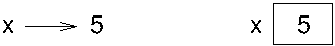
\includegraphics[width=2.5in]{figs/variables.pdf}}
%\caption{Diagrams that represent variables in Python (left) and
%C (right).}
%\label{variables}
%\end{figure}



\section{编译流程}

作为程序员, 你应该对编译期间发生了什么有个大致脉络.
如果你熟悉这个过程, 便可以帮你了解错误信息, 调试代码, 
以及避免常见的陷阱.


编译步骤如下:

\begin{enumerate}

\item 预处理: C 是一种包括 {\bf 预处理指令} 的语言, 
  这些指令是在编译之前起效的. 比如, \verb"#include" 指令会
  将另一个文件的源代码插入到指令的位置.

\item 解析: 解析期间, 编译器会读取源码并构建程序的内在结构, 也
  就是{\bf 抽象语法树}. 在此期间检查出来的错误, 通常是语法错误.

\item 静态检查: 编译器会检查变量和值的类型是否正确, 
  调用函数是否使用了正确数量和类型的参数, 等等.
  此阶段侦测到的错误通常是 {\bf 静态语义} 错误.

\item 代码生成: 编译器会读取程序的内在结构, 
  并生成机器码或字节码.

\item 链接: 如果程序使用了库中定义的值和函数, 
  编译器需要找到合适的库, 并囊括所需的代码.

\item 优化: 在整个流程的各个阶段, 编译器可以转换程序, 生成
  运行更快, 或更加节约空间的代码. 大部分的优化是一些简单的修改, 可以消除
  明显的耗费, 但有些编译器可以执行更复杂的分析和代码转换.

\end{enumerate}

通常运行{\tt gcc}时, 它会执行所有这些步骤, 生成一个可执行文件.
比如, 下面是一个极简的C程序代码:

\begin{verbatim}
#include <stdio.h>
int main()
{
    printf("Hello World\n");
}
\end{verbatim}

如果你将上述代码保存为一个名为{\tt hello.c}的文件, 
你便能像这样对其进行编译和执行:

\begin{verbatim}
$ gcc hello.c
$ ./a.out
\end{verbatim}

默认情况下, {\tt gcc} 将可执行代码存储在名为 {\tt a.out}
(起初表示``assembler output'')的文件中.
第二行会运行可执行文件. 
前缀 \verb"./"是告诉shell在当前目录中查找.

通常最好使用{\tt -o} 标识为可执行文件提供一个合适的名称:

\begin{verbatim}
$ gcc hello.c -o hello
$ ./hello
\end{verbatim}


\section{目标码}

使用{\tt -c}标识, 可以令{\tt gcc}编译程序并生成机器码, 但并不会链接库中函数, 也就不会生成可执行文件:

\begin{verbatim}
$ gcc hello.c -c
\end{verbatim}

结果是一个名为{\tt hello.o}的文件, 其中{\tt o}表示
{\bf 目标码}, 也就是编译后的程序. 
目标码不可执行, 但可以链接到可执行文件中.

UNIX 命令{\tt nm} 可以读取目标文件, 并生成涉及其所定义和应用的
名称的信息. 例如:

\begin{verbatim}
$ nm hello.o
0000000000000000 T main
                 U puts
\end{verbatim}

输出结果表明{\tt hello.o}定义了名称{\tt main}, 以及名
为{\tt puts}的函数, 这个名字表示``put string''.
在这个例子中, {\tt gcc} 通过将庞大复杂的{\tt printf}函数,
替换为相对简单的{\tt puts}, 以进行优化.

你可以使用{\tt -O}标识来控制{\tt gcc}进行多大程度的优化.
默认情况下, 它优化得很少, 这会令调试相对简单.
而选项{\tt -O1}会开启常用且安全得优化.
更高得数字会开启更多得优化, 而这也就会需要更长得编译时间.

理论上, 优化除了加速程序之外, 不应该改变程序的行为. 
但如果你的程序存在微妙的错误, 那你可能会发现, 优化会令错误暴露
或消失. 通常在开发新代码时, 最好关闭优化.
一旦程序正常运行, 并能通过适当的测试, 你便可以
开启优化, 并确认测试仍然通过.


\section{汇编码}

类似于{\tt -c}标识, {\tt -S} 标识会令{\tt gcc}编译程序并生成
汇编码, 而这基本上是一种人可读的机器码形式.

\begin{verbatim}
$ gcc hello.c -S
\end{verbatim}

结果是一个名为{\tt hello.s}的文件, 看起来像这样:

\begin{verbatim}
        .file        "hello.c"
        .section     .rodata
.LC0:
        .string      "Hello World"
        .text
        .globl       main
        .type        main, @function
main:
.LFB0:
        .cfi_startproc
        pushq %rbp
        .cfi_def_cfa_offset 16
        .cfi_offset 6, -16
        movq %rsp, %rbp
        .cfi_def_cfa_register 6
        movl $.LC0, %edi
        call puts
        movl $0, %eax
        popq %rbp
        .cfi_def_cfa 7, 8
        ret
        .cfi_endproc
.LFE0:
        .size        main, .-main
        .ident       "GCC: (Ubuntu/Linaro 4.7.3-1ubuntu1) 4.7.3"
        .section     .note.GNU-stack,"",@progbits
\end{verbatim}

{\tt gcc} 通常会被设置, 为你运行的机器生成相应的代码,
所以对我来说, 它会生成x86汇编语言,
这可以在Intel, AMD 和其他厂商的多种处理器上运行.
如果你在不同架构上运行, 你可能会得到不同的代码.


\section{预处理}

现在我们在编译过程中向后再走一步.
你可以用{\tt -E}标识, 仅仅只运行预处理器:

\begin{verbatim}
$ gcc hello.c -E
\end{verbatim}

结果是预处理器的输出.
这个例子中, 它包含了{\tt stdio.h}中包含的代码, 
以及{\tt stdio.h}中包含的所有文件, 依此类推.
在我的机器上, 结果有800多行代码.
由于几乎每个C程序都包括{\tt stdio.h}, 所以这800行代码会被编译多次.
如果像很多C程序一样, 你也包含了{\tt stdlib.h},
那么结果要超过1800行代码了.


\section{理解错误}

现在我们知道了编译过程的各个步骤, 
便更容易理解错误信息了.
比如, 如果\verb"#include" 指令中存在错误, 
你会从预处理器得到下面这条信息:

\begin{verbatim}
hello.c:1:20: fatal error: stdioo.h: No such file or directory
compilation terminated.
\end{verbatim}

如果存在语法错误, 你会从编译器得到下面信息:

\begin{verbatim}
hello.c: In function 'main':
hello.c:6:1: error: expected ';' before '}' token
\end{verbatim}

如果使用了任何标准库都没有定义的函数,
你会从链接器得到下面错误信息:

\begin{verbatim}
/tmp/cc7iAUbN.o: In function `main':
hello.c:(.text+0xf): undefined reference to `printff'
collect2: error: ld returned 1 exit status
\end{verbatim}

{\tt ld}是UNIX链接器的名称, 
如此命名是因为``loading'' 是编译过程中和链接关系密切的另一步骤.

一旦程序运行, C 便几乎不会进行运行时检查,
所以你可能只会看到极少的运行时错误.
如果你除以零, 或者执行了其他非法的浮点操作, 
你会得到一个``Floating point exception(浮点异常).''
同时, 如果你尝试读取或写入一个错误的内存位置,
你会遇到 ``Segmentation fault(段错误).''

% TODO: -Wall and lint


\chapter{进程}

\section{抽象和虚拟化}

在我们谈论进程之前, 我想先定义几个词汇:

\begin{itemize}

\item 抽象: 抽象是某个复杂事物的简化表达.
例如, 当你开车时, 你知道当你左转方向盘时, 车会左转,
反之亦然. 当然, 方向盘连接着一系列机械和(通常是)液压系统, 
这些会使车轮转动, 同时车轮会以复杂的方式和路面互动.
作为一个司机, 你通常无需考虑这些细节. 你只需要一个
简单的逻辑模型来进行驾驶. 你的这个逻辑模型便是一种抽象.

同样地, 当你使用网络浏览器时, 你知道当你点击链接时,
浏览器会显示该链接所指的页面.
使这一切成为可能的软件和网络通信是复杂的.
但作为一个用户, 你不必了解其细节.

软件工程中一个重要部分就是设计想这样的抽象,
这些抽象可以使用户和其他程序员能够使用强大而复杂的系统,
而无需了解其实现的细节.

\item 虚拟化: 一种重要的抽象便是虚拟化, 这是创建一个令人满意的幻觉的过程.

例如, 很多公共图书馆会参与图书馆之间的协作, 允许其相互借书.
当我请求一本图书时, 有时这本书是在我当地的图书馆的书架上,
但其他时候, 它需要从另外的地方转移过来.
无论哪种情况, 当书籍可以领取时, 我都会接到通知.
我不必知道它来自哪里, 我也不需要知道我的图书馆里有哪些书.
整个系统创建了一个假象, 让我相信我的图书馆拥有世界上的任意一本图书.

我当地的图书馆里实际可用的书可能很少,
但对我来说, 可用的虚拟书籍包括合作的图书馆中的每一本书.

再举个例子, 大多数计算机只连接到一个网络, 
但该网络会连接到其他网络, 依此类推.
我们所称的互联网是一组网络和协议, 
它们可以将数据包从一个网络转发到下一个网络. 
从用户或程序员的角度来看, 
该系统表现得好像互联网上的每台计算机都与其他计算机相连. 
所以物理连接的数量虽然很少, 但虚拟连接的数量是非常大的.

\end{itemize}

``虚拟''一词通常在虚拟机的上下文中使用, 虚拟机是一种软件, 会给你一种假象,
彷佛你运行在一个运行着特定操作系统的专有机器上.
而实际上, 虚拟机可能和很多其他虚拟机一起运行在同一台计算机上, 这些虚拟机可能运行着
不同的操作系统.

在虚拟化的上下文中, 我们有时称真实发生的事情为``物理事件'', 
而虚拟发生的事情为``逻辑事件''或者``抽象事件''.


\section{隔离}

工程学最重要的一个原则便是隔离:
当你设计一个包括多个部件的系统时, 最好将其相互之间进行隔离,
如此一个部件的改变就不会给其他组件带来不良影响.

操作系统的一个重要目标便是将每个运行的程序和其他程序进行隔离,
如此程序员便无需关注任何交互的可能.
提供这种隔离性的软件对象叫做{\bf 进程}.

进程是一个表示当前运行程序的软件对象.
我说的``软件对象''是指面向对象编程中的对象;
通常, 对象包含数据以及操作数据的方法.
一个进程便是一个包含下面数据的对象:

\begin{itemize}

\item 程序的文本, 通常是一系列机器语言指令.

\item 程序相关的数据, 包括静态数据(编译时分配)和动态数据(运行时分配).

\item 任何未完成的输入/输出操作的状态. 比如, 
  如果进程正在等待从磁盘读取数据, 或者等待网络数据到达, 
  这些操作的状态便是进程的一部分.

\item 程序的硬件状态, 包括寄存器中的数据, 状态信息以及程序计数器.
  程序计数器用来标识当前正在执行哪个指令.

\end{itemize}

通常一个进程运行一个程序, 但也可能会加载并运行新的程序.

还有可能, 也是很常见的情况是, 
多个进程中运行同一个程序. 在这种情况下, 这些进程会共享相同的程序代码,
但通常数据和硬件状态不同.

多数操作系统会提供一组基础功能, 以使进程之间相互隔离:

\begin{itemize}

\item 多任务: 多数操作系统都具有一种能力,
  可以在任何时刻将运行中的进程中断, 并保存其硬件状态,
  然后稍后恢复进程.
  通常, 程序员不必考虑这些中断.
  程序的行为就像在专用处理器上连续运行一样,
  只是指令之间的时间是不可预测的.

\item 虚拟内存: 多数操作系统都会创建这样的假象, 
  即每个进程都有自己的一段空间, 与其他进程都隔离开来.
  同样地, 程序员一般无需关注虚拟内存如何工作; 
  他们可以按照每个程序都有一段专门的内存来进行操作.

\item 设备抽象: 运行在同一个计算机上的进程, 共享磁盘驱动器, 网络接口, 
  图形卡, 以及其他硬件. 如果进程不经协商便直接和硬件交互, 便会引发混乱.
  例如, 本来要传递给某个进程的网络数据, 可能被其他进程读取, 
  或多个进程向硬盘上同一个位置存储数据.
  这便有赖于操作系统提供适当的抽象, 以维护秩序.

\end{itemize}

作为程序员, 你并不需要知道这些功能实现的详情.
但如果你有兴趣, 你会发现在各种隐喻之下, 
有很多有趣的事情正在发生.
如果你知晓发生的细节, 那你将成为更好的程序员.


\section{UNIX 进程}
\label{unixps}

当写这本书时, 我最关注的进程是我的文本编辑器, emacs.
每隔一段时间, 我会切换到终端窗口.
这是一个运行 UNIX shell 的窗口, 它提供了命令行界面.

当我移动鼠标, 窗口管理器便会被唤醒, 查看鼠标是否在终端窗口上,
然后又会唤醒终端. 终端唤醒shell. 
如果我在shell中输入{\tt make}, 
它会创建一个新的进程来执行 Make, 创建另一个进程运行 LaTeX,
然后再创建一个进程来显示结果.

如果我需要查找一些东西, 我可能会切换到另一个桌面,
这也会再次唤醒窗口管理器.
如果我点击网络浏览器的图标, 窗口管理器会创建一个进程, 运行网络浏览器.
有些浏览器, 比如 Chrome, 会为每个窗口和每个标签页都创建新的进程.

这些还只是我知道的进程.
同时, 还有很多其他进程在{\bf 后台} 运行.
其中很多进程正在执行与操作系统相关的操作.

UNIX 命令 {\tt ps} 可以打印正在运行的进程的信息.
如果你在终端执行它, 你可能会看到像这样的东西:

\begin{verbatim}
  PID TTY          TIME CMD
 2687 pts/1    00:00:00 bash
 2801 pts/1    00:01:24 emacs
24762 pts/1    00:00:00 ps
\end{verbatim}

第一列是唯一的数字格式进程ID.
第二列是创建进程的终端; 
``TTY''代表电传打印机, 这是最早的机械终端.

第三列是进程使用的处理器总时间, 以小时、分钟和秒为单位.
在这个例子中, {\tt bash} 是解释输入命令的 shell 的名称,
emacs 是我的文本编辑器, ps 是生成此输出的程序.

默认情况下, {\tt ps} 仅列出和当前终端相关的进程.
如果你使用{\tt -e} 标志, 你便能获取每个进程(包括属于其他用户的进程,
就我看来, 这是一个安全漏洞).

在我的系统上, 目前有233个进程.
下面是其中一些:

\begin{verbatim}
  PID TTY          TIME CMD
    1 ?        00:00:17 init
    2 ?        00:00:00 kthreadd
    3 ?        00:00:02 ksoftirqd/0
    4 ?        00:00:00 kworker/0:0
    8 ?        00:00:00 migration/0
    9 ?        00:00:00 rcu_bh
   10 ?        00:00:16 rcu_sched
   47 ?        00:00:00 cpuset
   48 ?        00:00:00 khelper
   49 ?        00:00:00 kdevtmpfs
   50 ?        00:00:00 netns
   51 ?        00:00:00 bdi-default
   52 ?        00:00:00 kintegrityd
   53 ?        00:00:00 kblockd
   54 ?        00:00:00 ata_sff
   55 ?        00:00:00 khubd
   56 ?        00:00:00 md
   57 ?        00:00:00 devfreq_wq
\end{verbatim}

{\tt init} 是操作系统启动时创建的第一个进程.
它会创建许多其他进程, 然后闲置, 
直到它创建的进程都结束.

{\tt kthreadd} 是操作系统用来创建 {\bf 线程} 的进程.
后续我们将更详细地讨论线程, 当前你可以将线程看作是一种进程.
开头的{\tt k} 代表 {\bf 内核(kernel)},
这是操作系统符合核心功能(比如创建线程)的部分.
结尾的 {\tt d} 代表 {\bf 守护程序(daemon)},
这是运行在后台, 并提供操作系统服务的进程的另一个名称.
在此, ``daemon'' 是指一种乐于助人的精神, 没有任何邪恶的意思.
 
根据名称, 你可以推断出{\tt ksoftirqd} 也是一个内核守护程序;
具体来说, 它处理软件中断请求, 即 ``软中断(soft IRQ)''

{\tt kworker} 是一个内核创建的工作进程, 用来为内核处理一些任务.

通常有多个进程运行着内核服务.
在我的系统上, 现在有8个{\tt ksoftirqd} 进程和35个{\tt kworker} 进程.

我不会详细讨论其他进程, 但如果你感兴趣, 
你可以搜索更多关于它们的信息.
你应该在你的系统上运行 {\tt ps}, 并将结果和我的进行对比.

%TODO: using gdb here?


\chapter{虚拟内存}

\section{一点信息论知识}

{\bf 比特(bit)} 是一个二进制的数位, 也是一个信息单元.
如果你有一比特, 便可以表示两种可能性中的一种, 通常写作 0 和 1.
如果你有两比特, 那边有4种组合, 分别是 00, 01, 10, 和 11.
通常, 如果你有 $b$ 个比特, 你便可以表示 $2^b$个值.
一个{\bf 字节(byte)} 是8个比特, 所以可以表示256个值.

反过来想, 假设你想储存一个字母. 字母表有26个字母, 
那么你需要几个比特呢? 如果用4个比特, 你可以表示16个值, 数量不够.
如果用5个比特, 你可以表示多达32个值, 这足够表示所有字母了, 而且还有剩余.

通常, 如果你想表示$N$个值, 你应该选择满足 $2^b \ge N$ 的最小 $b$ 值.
两侧以2为底取对数, 便可以得到 $b \ge log_2 N$.

假设我掷一枚硬币, 并告诉你结果, 那么我便是给了你一比特的信息.
如果我掷一个六面骰子, 并告诉你结果, 那我便是给了你 $log_2 6$ 个比特的信息.
通常, 如果发生的概率是$N$中的1个, 那么结果便包含 $log_2 N$ 个比特信息.

同样的, 如果结果出现的概率是 $p$, 那么信息量便是 $-log_2 p$.
这个数量也被称为结果的{\bf 自信息}, 它是用来衡量结果的惊奇程度, 
所以也被称为{\bf 惊奇度}. 如果你的马仅有$1/16$的概率获胜,
但是赢了, 你可以4比特的信息(以及赔付). 
但如果获胜的机率是75\%, 那么胜利的消息只包含0.42比特.

直观来说, 出乎意料的消息反而包含了大量的信息.
相反, 如果你已经确定某件事情, 那么证实它仅会提供少量信息.

在本书的诸多主题中, 我们需要在比特数, $b$, 和其能编码的值的数量 $N = 2^b$ 之间
熟练转换.


\section{内存和存储}

进程运行时, 其大部分数据存储在{\bf 主内存}, 这通常是一种随机访问存储(RAM).
当前多数计算机上, 主存储都是{\bf 易失的}, 也就意味着一旦计算机关机, 
主存储的内容便会丢失. 一台典型的桌面计算机有 2--8 GiB 内存.
GiB 表示``gibibyte,'' 也就是 $2^{30}$ 字节.

进程需要读写文件, 而文件往往存储在硬盘驱动器(HDD)或者固态硬盘中.
这些存储设备都是 {\bf 非易失的}, 因此可以用作长期存储.
目前一台典型桌面计算机会拥有500GB到2TB容量的硬盘.
其中GB表示``gigabyte,'' 也就是 $10^9$ 字节.
TB 表示 ``terabyte,'' 也就是 $10^{12}$ 字节.

你可能已经注意到, 我描述主内存大小时, 用二进制单位GiB,
描述硬盘大小时, 用十进制单位GB和TB.
由于一些历史和科技的原因, 内存通常用二进制单位衡量, 而硬盘则用十进制单位.
在本书中, 我将谨慎区分二进制和十进制单位,
但你也应该注意到, ``gigabyte''和缩写GB通常是混用的.
% gibabyte 不是等于GB吗,还是想表达 gibibyte 和GB?

在非正式的使用中, ``内存''一词有时候会指 HDD和SSD, 以及 RAM. 但
这些设备的属性是不同的, 所以我们需要仔细区分它们. 我将使用
{\bf 存储} 来指代 HDD和SSD.


\section{地址空间}

主内存中的每个字节都由一个整数{\bf 物理地址}指定.
有效的物理地址集被称为物理{\bf 地址空间}.
通常从0 到 $N-1$, 其中$N$ 是内存的大小.
在1 GiB 物理内存的系统上, 最高的有效地址是$2^{30}-1$, 
即十进制下的1,073,741,823 , 或者十六进制下的0x3fff ffff(前缀的 0x 表示十六进制数).

然而, 大部分的操作系统会提供{\bf 虚拟内存}, 这意味着程序永远不必处理
物理地址, 也不必知道由多少物理地址可用.

相反, 程序会使用从 0 到 $M-1$ 编号的{\bf 虚拟地址}, 其中$M$ 是有效
虚拟地址的数量. 虚拟地址空间的大小是由操作系统和其运行的硬件共同决定的.

你可能听锅别人谈论32位系统和64位系统.
这些术语表示的是寄存器的大小, 通常也是虚拟地址的大小.
在32位系统上, 虚拟地址为32位, 也就是虚拟地址空间从0到0xffff ffff.
所以地址空间的大小为$2^{32}$字节, 或 4 GiB.

而在64位系统上, 虚拟地址空间是$2^{64}$字节, 或$2^4 \cdot 1024^6$ 字节.
这是16 exbibytes, 约为当前物理内存的十亿倍.
虚拟地址空间比物理内存大这么多, 这看起来很奇怪, 但是我们稍后就会看到它是
如何工作的.

当程序从内存读取或者向内存写入值时, 它会生成虚拟地址.
在操作系统的帮助下, 访问内存之前, 硬件会被转换成物理地址.
这种转换是基于每个进程进行的, 所以即使两个进程生成同样的虚拟地址,
它们也会映射到物理内存的不同位置.

最后, 虚拟内存是操作系统隔离进程的一种重要手段.
通常, 一个进程是无法访问另一个进程拥有的数据的, 
因为如果某块物理内存已经被分配给了其他进程,
那么该进程便无法生成映射到这块物理内存的虚拟地址.


\section{内存段}

运行中得进程的数据会被组织成五个段:

\begin{itemize}

\item {\bf 代码段} 包含程序文本; 也就是构成程序的机器语言指令.

\item {\bf 静态段} 包含不可变的值, 像字符串常量. 比如, 如果你的程序包含
字符串{\tt "Hello, World"}, 那这些字符会被保存在静态段.

\item {\bf 全局段} 包含全局变量和被声明为{\bf static(静态类型)}的
局部变量.

\item {\bf 堆段} 包含运行时被分配的内存块, 通常是通过调用C库函数
{\bf malloc}所分配.

\item {\bf 栈段} 包含调用栈, 也就是一系列的堆栈帧.
每次函数被调用, 都会为其分配一个包含函数的参数和局部变量的堆栈帧.
当函数运行结束, 其堆栈帧会从栈中移除. 

\end{itemize}

段的排序部分由编译器决定, 部分由操作系统决定.
具体细节取决于操作系统, 但常见的排列方式包括::

\begin{itemize}

\item 文本段位于内存接近``底部''的位置, 也就是靠近地址0的地方.

\item 静态段通常在文本段上方, 也就是高地址位置.

\item 全局段通常位于静态段上方.

\item 堆通常在全局段上方. 随着堆的扩张, 它会向更大地址增长.
  
\item 栈靠近内存的顶部; 也就是虚拟地址空间中最高地址附近.
栈扩展时, 会朝着更小地址方向增长.

\end{itemize}

%TODO: Figure out how to handle the code that is in both ExercisesInC
% and the repo for the book.

若要确定你系统上这些段的布局, 尝试运行这个程序,在本书仓库
中的 {\tt aspace.c} 文件中(详见第~\ref{code}节). 


\begin{verbatim}
#include <stdio.h>
#include <stdlib.h>

int global;

int main ()
{
    int local = 5;
    void *p = malloc(128);
    char *s = "Hello, World";

    printf ("Address of main is %p\n", main);
    printf ("Address of global is %p\n", &global);
    printf ("Address of local is %p\n", &local);
    printf ("p points to %p\n", p);
    printf ("s points to %p\n", s);
}
\end{verbatim}

{\tt main}是这个函数的名称; 当作为变量使用时, 
它指的是{\tt main}中的第一条机器语言指令的地址, 
同时我们希望它在文本段中.

{\tt global} 是全局变量, 所以我们希望它在全局段中. 
{\tt local} 是局部变量, 我们期望它存在于栈中.

{\tt s} 指向``字符串文本'', 它是程序的一部分(与从文件读取, 
或用户输入的字符串等不同). 我们希望字符串的位置在静态段中(与指针
{\tt s}不同, 它是局部变量).

{\tt p} 包含{\tt malloc}返回的地址, 
这个函数会在堆中分配空间. ``malloc'' 表示 ``memory allocate(内存分配)''.

格式序列\verb"%p" 会告诉{\tt printf}将每个地址格式化为``指针'',
因此它会以十六进制显示结果.

当我运行这个程序, 输出如下(我增加了些空格,以便于阅读):


\begin{verbatim}
Address of main is   0x      40057d
Address of global is 0x      60104c
Address of local is  0x7ffe6085443c
p points to          0x     16c3010
s points to          0x      4006a4

\end{verbatim}

和预计的一样, {\tt main} 的地址是最低的, 然后是字符串文本的位置.
接着是{\tt global}的位置, 再然后是{\tt p}指向的地址.
{\tt local}的地址要大得多.

最大的地址有12位十六进制数. 每个十六进制数对应4个比特,
所以一共是48比特地址. 这便表示可用虚拟地址空间的大小为$2^{48}$字节.

做个练习, 在你电脑上运行这个程序, 并和我的结果进行比较.
再添加一个 {\tt malloc}, 检查你系统上的堆是否向上增长了(向更大地址方向).
再添加一个输出局部变量地址的函数, 并检查栈是否向下变化了.


\section{静态局部变量}

栈上的局部变量有时被称为{\bf 自动变量},
因为它们会在函数调用时, 自动分配, 在函数返回时, 自动释放.

在C语言中, 存在另一种局部变量, 会在全局段中进行分配, 称为{\bf 静态变量},
它会在程序启动时被初始化, 同时在函数调用之间保持其值不变.

例如, 下面的函数会跟踪其被调用的次数.

\begin{verbatim}
int times_called()
{
    static int counter = 0;
    counter++;
    return counter;
}
\end{verbatim}

关键字{\tt static}表示 {\tt counter} 是一个静态局部变量.
初始化仅会在程序启动时, 发生一次.

如果你将此函数添加到{\tt aspace.c}中, 你便可以确认{\tt counter}是在全局段中
与全局变量一起分配的, 而不是在栈中分配的.
% If you add this function to {\tt aspace.c} you can confirm that
% need a full point. 需要一个句号



\section{地址转换}
\label{address_translation}

虚拟地址(VA) 如何能转换成物理地址(PA)?
基本机制很简单, 但简单的实现会太慢, 并消耗太多空间.
所以实际的实现有点复杂.

\begin{figure}
\centerline{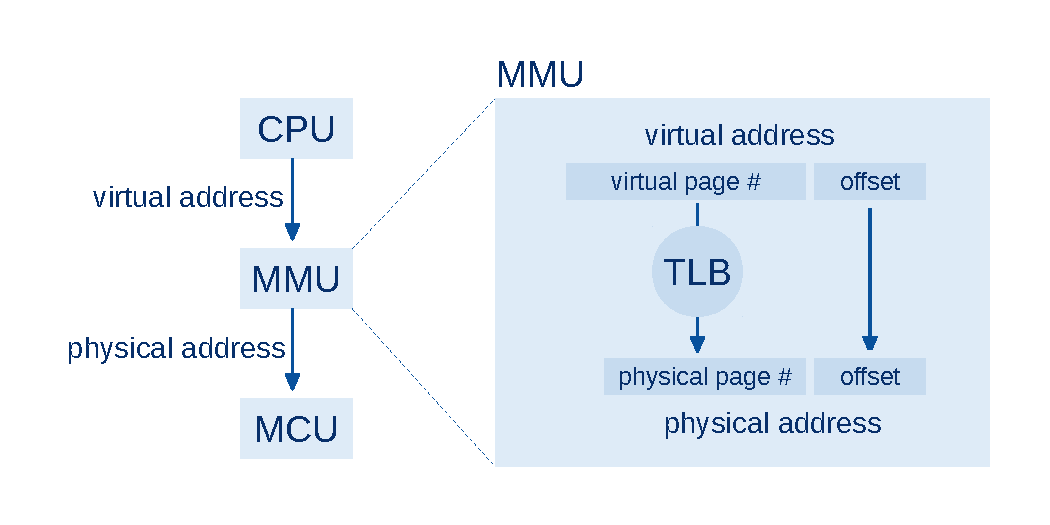
\includegraphics[width=3in]{figs/address_translation.pdf}}
\caption{地址转换过程示意图.}
\label{addtrans}
\end{figure}

大部分处理器会提供位于CPU和主存之间的内存管理单元(MMU).
MMU 会执行VA和PA之间的快速转换.

\begin{enumerate}

\item 当程序读取或写入一个变量时, CPU会生成一个VA.

\item MMU 将VA 分成两部分, 分别是页号和偏移量.
``页''是内存的一个块, 页的大小取决于操作系统和硬件, 常见大小一般是 1--4 KiB.

\item MMU会从页表缓存 (TLB) 查找页号, 并获得相应的物理地址页号.
然后, 它将物理页号和偏移量结合起来, 构成PA.

\item PA 会传递给主存, 主存基于给定位置进行读写.

\end{enumerate}

TLB 包含来自页表(存储在内核内存中)数据的缓存副本.
页表包含虚拟页号到物理页号的映射. 
由于每个进程都有自己的页表, 因此TLB必需确保它只使用正在运行的进程的页表中的条目.

图~\ref{addtrans} 是这个过程的示意图.
若要明了其工作原理, 假设VA是32位, 物理内存是 1 GiB, 并划分为了 1 KiB 的页.

\begin{itemize}

\item 因为 1 GiB 是 $2^{30}$ 字节, 1 KiB 是 $2^{10}$ 字节, 
  所以有 $2^{20}$ 个物理页, 有时也称为 ``帧''.

\item 虚拟地址空间大小是 $2^{32}$ B, 单个页的大小是 $2^{10}$ B, 
  所以有 $2^{22}$ 个虚拟页.

\item 偏移量的大小由页面大小决定.  这个例子中, 页面大小是 $2^{10}$ B, 
  所以需要10位来定位页面上的字节.

\item 如果 VA 是 32 位, 同时偏移量是 10 位, 剩下的22位便构成了虚拟页号.

\item 由于有 $2^{20}$ 个物理页, 每个物理页号是20位. 
  加上10位的偏移量, 得到的 PA 便是 30 位.

\end{itemize}

至此, 一切似乎看起来可行. 但让我们想一下, 页表可能有多大.
页表的最简单实现是一个数组, 其中每个条目对应一个虚拟页.
每个条目包含物理页号, 本例中是20位, 以及关于每帧的附加信息.
所以我们预计每个条目需要3--4字节的空间.
由于存在$2^{22}$个虚拟页, 
页表将需要$2^{24}$字节, 即 16 MiB.

由于每个进程都需要一个页表, 
那么运行256个进程的系统, 便需要$2^{32}$字节, 即 4GiB, 还只是页表空间!
而这仅仅是针对32位虚拟地址的情况.
对于48-或64-位的虚拟地址来说, 这个数字就太吓人了.

幸运的是, 我们实际上并不需要这么多空间,
因为多数进程甚至用不到虚拟地址空间的一小部分.
而且, 如果一个进程不使用虚拟页, 我们便不需要在页面中为其分配条目.

另一种表达同样观点的方式是页表是``稀疏的'',
而这最简单的实现方式, 即一个页表条目数组, 但这是一个糟糕的注意.
幸运的是, 对于稀疏数组, 有其他高效的实现方案.

一种选择是多级页表, 这是许多操作系统(包括Linux)使用的方案.
另一种选择是关联表, 其中每个条目包括虚拟页号和物理页号.
在软件中检索关联表很慢, 但在硬件中, 我们可以并行检索整个表,
所以其通常用于表示TLB中的页表条目.

你也可以从\url{http://en.wikipedia.org/wiki/Page_table}了解更多关于这些实现的信息;
你可能对这些细节感兴趣.
但核心思想为页表是稀疏的, 所以我们需要为稀疏数组选择一个好的实现方案.

前面我提到操作系统可以中断运行中的进程, 保存其状态, 然后运行另一个进程.
这个机制叫做{\bf 上下文切换}. 因为每个进程都有自己的页表, 操作系统需要和MMU协作,
从而确保每个进程都能获得正确的页表.
在老的机器上, MMU中的页表信息需要在每次上下文切换时进行替换, 
而这是很昂贵的.
在新的系统中, MMU 中的每个页表条目都包含进程ID, 因此多个进程的页表可以同时存在于MMU中.


\chapter{文件和文件系统}

当进程结束(或崩溃), 存储在主内存中的任何数据都会丢失.
但存储在硬盘驱动器(HDD)或者固态硬盘驱动器上的数据是``持久的'';
也就是说进程结束, 甚至计算机关闭, 也会存在.

硬盘驱动器是复杂的, 数据以块的形式存储, 
这些块存在于扇区上, 扇区构成磁道, 
磁道则排列在盘片的同心圆上.

固态硬盘在某种意义上相对简单, 
因为块会按照顺序编号, 但它们也因此引入了一个不一样的复杂性:
每个块只能写入有限的次数, 然后就会变得不可靠.

作为个程序员, 你不会想要处理这些复杂性.
你想要的是对持久存储硬件的合理抽象.
而最常见的抽象就是``文件系统''.

抽象地说:

\begin{itemize}

\item ``文件系统''是将每个文件名称映射到其内容的一种方式.
如果你将名称视为键, 内容当作值, 文件系统便是一种键-值数据库.
(参见 \url{https://en.wikipedia.org/wiki/Key-value_database}).

\item  一个``文件'' 便是一个字节序列.

\end{itemize}

文件名通常为字符串, 而且一般是``分层次的'';
也就是说, 该字符串指定了一个从顶级目录(或文件夹)到特定文件的一系列子目录的路径.

抽象层以及底层机制之间最主要的区别是, 文件是基于字节的, 而持久层存储是基于块的.
操作系统将C库中基于字节的文件操作转换为对存储设备上基于块的操作.
典型的块大小一般为1--8 KiB.

例如, 下面代码会打开文件并读取第一个字节:

\begin{verbatim}
    FILE *fp = fopen("/home/downey/file.txt", "r");
    char c = fgetc(fp);
    fclose(fp);
\end{verbatim}

上述代码运行时:

\begin{enumerate}

\item {\tt fopen} 会使用文件名中的\verb"/" 确定顶级目录, 
  以及子目录{\tt home}, 以及下一级子目录 {\tt downey}.

\item 它会找到名为{\tt file.txt}的文件, 然后``打开(opens)''文件以进行读取,
  也就表示, 这会创建一个表示正在被读取的文件的数据结构.
  这个数据结构除了其他事情, 还会跟踪文件已读取了多少, 也就是``文件位置''.
  
  在DOS中, 这个数据结构叫做文件控制块(FCB), 但我希望尽量避免使用这个术语,
  因为在UNIX中, 它有其他含义. 在UNIX中, 似乎没有一个相应的好名称. 它是
  打开文件表中的一个条目, 所以我称其为打开文件表条目.

\item 当我调用{\tt fgetc}时, 操作系统会检查文件的下一个字符是否已经存在于
  内存中. 如果已存在, 则会读取下一个字符, 更新文件位置, 并返回结果.

\item 如果下一个字符不在内存中, 操作系统会发出一个 I/O 请求, 获取下一个块.
  磁盘驱动器速度较慢, 所以一个等待从磁盘获取块的进程通常会被中断, 以便另一个进程运行,
  直到数据返回, 再回到等待的进程.

\item 当 I/O 操作结束, 新的数据块会被存储到内存, 同时进程继续运行. 读取第一个字符,
  并将其存储为局部变量.

\item 当进程关闭文件, 操作系统会完成或者取消所有挂起的操作, 移除存储在内存中的数据,
  并释放打开文件表条目(OpenFileTableEntry).

\end{enumerate}

写文件的过程类似, 只是会多一些额外步骤. 
下面是一个打开文件进行写入并修改第一个字符的示例.

\begin{verbatim}
    FILE *fp = fopen("/home/downey/file.txt", "w");
    fputc('b', fp);
    fclose(fp);
\end{verbatim}

当代码运行时:

\begin{enumerate}

\item 再次, {\tt fopen} 使用文件名定位文件. 如果文件不存在, 则会创建
  一个新文件, 并在父目录{\tt /home/downey}中添加一个条目.

\item 操作系统会创建一个打开文件表条目, 以标明此文件以写入方式打开, 
  同时设置文件位置为 0.

\item {\tt fputc} 会尝试写入(或重写)文件的第一个字节. 如果文件已经存在,
  操作系统需要将第一个块加载入内存. 否则, 它会在内存中分配一个新块, 同时
  在磁盘上申请一个新块.

\item 内存中的块被修改后不会立刻被复制回磁盘. 通常, 写入文件的数据是``缓冲的'',
  意味着它会保存在内存, 直到至少有一个块需要写入, 才会写入磁盘.

\item 当文件关闭, 任何缓冲区的数据都会被写入磁盘, 同时释放打开文件表条目.

\end{enumerate}

综上所述, C 库提供了一个从文件名映射到字节流的文件系统的抽象. 
这个抽象建立在实际以块进行组织的存储设备之上.


\section{磁盘性能}

\newcommand{\mus}{$\mu$s~}

我之前提过磁盘驱动器很慢. 对于当前的HDD来说, 
从磁盘读取一个块到内存的平均时间大约5--25毫秒
(参见 \url{https://en.wikipedia.org/wiki/Hard_disk_drive_performance_characteristics}).
而SSD则快很多, 读一个 4 KiB的块, 只需要25 \mus, 写一个块需要250 \mus
(参见 \url{http://en.wikipedia.org/wiki/Ssd#Controller}).

为了更好地理解这些数字, 我们将其和CPU的时钟周期进行比较.
时钟频率为 2GHz的处理器每0.5 ns完成一个时钟周期.
从内存获取一个字节到CPU的时间通常约为100 ns. 
如果处理器每个时钟周期完成一条指令, 那么在等待从内存获取一个字节的时间可以
完成200条指令.

在1微秒内, 处理器可以完成2000条指令, 
所以等待从SSD获取一字节的25 \mus 内, 可以完成 50,000 条指令.

在1毫秒内, 处理器可以完成 2,000,000 条指令,
所以等待从HDD获取一字节的20 ms内, 处理器可以完成4 千万条指令. 
如果在等待期间, CPU 没有其他任务执行, 则它会处于空闲状态.
这也是为什么操作系统通常在等待磁盘数据时切换到另一个进程的原因.

主存和持久化存储之间的性能差距是计算机系统设计的主要挑战之一.
操作系统和硬件提供了几种特性, 以 ``填补''这个差距:

\begin{itemize}

\item 块传输: 从磁盘加载单个字节的时间是5--25 ms.
  相比之下, 加载 8 KiB 块的额外时间可以忽略不急.
  所以系统通常每次访问磁盘时, 尽量读取大块数据.

\item 预取: 有时候操作系统可以预测一个进程将会读取的块, 从而在请求之前便进行加载.
  比如, 如果你打开一个文件并读取第一个块, 那么你很可能会继续读取第二个块.
  操作系统可能会在被请求之前, 先加载其他块.

\item 缓冲区: 正如我之前提到的, 当你写入一个文件, 操作系统会将数据存储在内存中,
  稍后再将其写入磁盘. 如果当其在内存中时, 你多次修改了块, 系统只需要往磁盘写入一次.

\item 缓存: 如果进程最近使用了某个块, 很可能再次使用它.
  如果操作系统在内存中保留了该块的副本, 那便可以以内存速度处理将来的请求.

\end{itemize}

这些功能的有些实现是在硬件中. 比如, 有些磁盘驱动器会提供一个缓存, 来存储最近使用过
的块, 同时很多磁盘驱动器即使只被请求了一个块, 也会一次夺取多个块.

这些机制通常会提高程序的性能, 但不会改变其行为.
通常程序员不需要考虑它们, 除非出现以下两种情况: 
(1)如果程序性能很糟糕, 你可能需要了解这些机制以便诊断问题, 以及
(2)当数据被缓冲存储了, 程序调试会变得困难. 
例如, 如果一个程序打印一个值, 然后崩溃. 该值可能不会出现, 因为它可能在缓冲区.
同样, 如果一个程序往磁盘写数据, 然后计算机断电了, 如果数据还在缓存中, 尚未
写入磁盘, 那么数据很可能会丢失.


\section{磁盘元数据}

The blocks that make up a file might be arranged contiguously on
disk, and file system performance is generally better if they are,
but most operating systems don't require contiguous allocation.
They are free to place a block anywhere on disk, and they use
various data structures to keep track of them.

In many UNIX file systems, that data structure is called an ``inode,''
which stands for ``index node''.  More generally, information about
files, including the location of their blocks, is called ``metadata''.
(The content of the file is data, so information about the file is
data about data, hence ``meta''.)

Since inodes reside on disk along with the rest of the data, they are
designed to fit neatly into disk blocks.  A UNIX inode contains
information about a file, including the user ID of the file owner;
permission flags indicating who is allowed to read, write, or execute
it; and timestamps that indicate when it was last modified and
accessed.  In addition, it contains block numbers for the first 12
blocks that make up the file.

If the block size is 8 KiB, the first 12 blocks make up 96 KiB.
On most systems, that's big enough for a large majority of files,
but it's definitely not big enough for all of them.  That's
why the inode also contains a pointer to an ``indirection block'',
which contains nothing but pointers to other blocks.

The number of pointers in an indirection block depends on the sizes of
the blocks and the block numbers, but it is often 1024.  With 1024
block numbers and 8 KiB blocks, an indirection block can address 8
MiB.  That's big enough for all but the largest files, but still not
big enough for all.

That's why the inode also contains a pointer to a ``double indirection
block'', which contains pointers to indirection blocks.  With
1024 indirection blocks, we can address 8 GiB.

And if that's not big enough, there is (finally) a triple indirection
block, which contains pointers to double indirection blocks, yielding
a maximum file size of 8 TiB.  When UNIX inodes were designed, that
seemed big enough to serve for a long time.  But that was a long time
ago.

As an alternative to indirection blocks, some files systems, like FAT,
use a File Allocation Table that contains one entry for each block,
called a ``cluster'' in this context.  A root directory contains a
pointer to the first cluster in each file.  The FAT entry for each
cluster points to the next cluster in the file, similar to a linked
list.  For more details, see
\url{http://en.wikipedia.org/wiki/File_Allocation_Table}.


\section{Block allocation}

File systems have to keep track of which blocks belong to each file;
they also have to keep track of which blocks are available for use.
When a new file is created, the file system finds an available
block and allocates it.  When a file is deleted, the file system
makes its blocks available for re-allocation.

The goals of the block allocation system are:

\begin{itemize}

\item Speed: Allocating and freeing blocks should be fast.

\item Minimal space overhead: The data structures used by the allocator
  should be small, leaving as much space as possible for data.

\item Minimal fragmentation: If some blocks are left unused, or some
  are only partially used, the unused space is called
  ``fragmentation''.

\item Maximum contiguity: Data that is likely to be used at the same
  time should be physically contiguous, if possible, to improve
  performance.

\end{itemize}

It is hard to design a file system that achieves all of these
goals, especially since file system performance depends on
``workload characteristics'' like file sizes, access
patterns, etc.  A file system that is well tuned for one workload
might not perform as well for another.

For this reason, most operating systems support several kinds of file
systems, and file system design is an active area of research and
development.  In the last decade, Linux systems have migrated
from ext2, which was a conventional UNIX file system, to ext3,
a ``journaling'' file system intended to improve speed and
contiguity, and more recently to ext4, which can handle larger files
and file systems.  Within the next few years, there might be
another migration to the B-tree file system, Btrfs.


\section{Everything is a file?}

The file abstraction is really a ``stream of bytes'' abstraction,
which turns out to be useful for many things, not just file systems.

One example is the UNIX pipe, which is a simple form of inter-process
communication.  Processes can be set up so that output from one
process is taken as input into another process.  For the first
process, the pipe behaves like a file open for writing, so it
can use C library functions like {\tt fputs} and {\tt fprintf}.
For the second process, the pipe behaves like a file open for
reading, so it uses {\tt fgets} and {\tt fscanf}.

Network communication also uses the stream of bytes abstraction.
A UNIX socket is a data structure that represents a communication
channel between processes on different computers (usually).  Again,
processes can read data from and write data to a socket using
``file'' handling functions.

Reusing the file abstraction makes life easier for programmers, since
they only have to learn one API (application program interface).
It also makes programs more versatile, since a program intended to
work with files can also work with data coming from pipes and other
sources.

% TODO: gprof here?


\chapter{More bits and bytes}

\section{Representing integers}

You probably know that computers represent numbers in
base 2, also known as binary.  For positive numbers, the binary
representation is straightforward; for example, the representation
for $5_{10}$ is $b101$.

For negative numbers, the most obvious representation uses
a sign bit to indicate whether a number is positive or negative.
But there is another representation, called ``two's complement''
that is much more common because it is easier to work with
in hardware.

To find the two's complement of a negative number, $-x$, find
the binary representation of $x$, flip all the bits, and add 1.
For example, to represent $-5_{10}$, start with the representation
of $5_{10}$, which is $b0000 0101$ if we write the 8-bit version.
Flipping all the bits and adding 1 yields $b1111 1011$.

In two's complement, the leftmost bit acts like a sign bit;
it is 0 for positive numbers and 1 for negative numbers.

To convert from an 8-bit number to 16-bits, we have to add
more 0's for a positive number and add 1's for a negative number.
In effect, we have to copy the sign bit into the new bits.
This process is called ``sign extension''.

In C all integer types are signed (able to represent positive and
negative numbers) unless you declare them {\tt unsigned}.  The
difference, and the reason this declaration is important, is that
operations on unsigned integers don't use sign extension.


\section{Bitwise operators}

People learning C are sometimes confused
about the bitwise operators \verb"&" and \verb"|".  These
operators treat integers as bit vectors and compute logical
operations on corresponding bits.

For example, \verb"&" computes the AND operation, which yields
1 if both operands are 1, and 0 otherwise.  Here is an example
of \verb"&" applied to two 4-bit numbers:
%
\begin{verbatim}
  1100
& 1010
  ----
  1000
\end{verbatim}
%
In C, this means that the expression \verb"12 & 10" has the
value 8.

Similarly, \verb"|" computes the OR operation, which yields
1 if either operand is 1, and 0 otherwise.
%
\begin{verbatim}
  1100
| 1010
  ----
  1110
\end{verbatim}
%
So the expression \verb"12 | 10" has the value 14.

Finally, \verb"^" computes the XOR operation, which yields
1 if either operand is 1, but not both.
%
\begin{verbatim}
  1100
^ 1010
  ----
  0110
\end{verbatim}
%
So the expression \verb"12 ^ 10" has the value 6.

Most commonly, \verb"&" is used to clear a set of bits from
a bit vector, \verb"|" is used to set bits, and \verb"^"
is used to flip, or ``toggle'' bits.  Here are the details:

{\bf Clearing bits}: For any value $x$, $x \& 0$ is 0, and $x \& 1$ is $x$.
So if you AND a vector with 3, it 
selects only the two rightmost bits, and sets the rest to 0.
%
\begin{verbatim}
  xxxx
& 0011
  ----
  00xx
\end{verbatim}
%
In this context, the value 3 is called a ``mask'' because it
selects some bits and masks the rest.

{\bf Setting bits}: Similarly, for any $x$, $x | 0$ is x, and $x | 1$ is $1$.
So if you OR a vector with 3, it sets the rightmost
bits, and leaves the rest alone:
%
\begin{verbatim}
  xxxx
| 0011
  ----
  xx11
\end{verbatim}
%
{\bf Toggling bits}: Finally, if you XOR a vector with 3, it flips the
rightmost bits and leaves the rest alone.  As an exercise, see if you
can compute the two's complement of 12 using \verb"^".  Hint: what's
the two's complement representation of -1?

% (12 ^ -1) + 1

C also provides shift operators, {\tt <<} and {\tt >>}, which shift
bits left and right.  Each left shift doubles a number, so
{\tt 5 << 1} is 10, and {\tt 5 << 2} is 20.  Each right shift
divides by two (rounding down), so {\tt 5 >> 1} is 2 and
{\tt 2 >> 1} is 1.


\section{Representing floating-point numbers}

Floating-point numbers are represented using the binary
version of scientific notation.  In decimal notation, large
numbers are written as the product of a coefficient and 10 raised
to an exponent.  For example, the speed of light in m/s is
approximately $2.998 \cdot 10^8$.

Most computers use the IEEE standard for floating-point
arithmetic.  The C type {\tt float} usually corresponds
to the 32-bit IEEE standard; {\tt double} usually corresponds
to the 64-bit standard.

In the 32-bit standard, the leftmost bit is the sign bit, $s$.
The next 8 bits are the exponent, $q$, and the last 23 bits are
the coefficient, $c$.  The value of a floating-point number is
%
\[ (-1)^s c \cdot 2^q \]
%
Well, that's almost correct, but there's one more wrinkle.
Floating-point numbers are usually normalized so that there is
one digit before the point.  For example, in base 10, we prefer
$2.998 \cdot 10^8$ rather than $2998 \cdot 10^5$ or any other
equivalent expression.  In base 2, a normalized number always
has the digit 1 before the binary point.  Since the digit in
this location is always 1, we can save space by leaving it
out of the representation.

For example, the integer representation of $13_{10}$ is $b1101$.
In floating point, that's $1.101 \cdot 2^3$, so the exponent
is 3 and the part of the coefficient that would be stored
is 101 (followed by 20 zeros).

Well, that's almost correct, but there's one more wrinkle.
The exponent is stored with a ``bias''.  In the 32-bit standard,
the bias is 127, so the exponent 3 would be stored as 130.

To pack and unpack floating-point numbers in C, we can use a 
union and bitwise operations.  Here's an example:
%
\begin{verbatim}
    union {
        float f;
        unsigned int u;
    } p;

    p.f = -13.0;
    unsigned int sign = (p.u >> 31) & 1;
    unsigned int exp = (p.u >> 23) & 0xff;

    unsigned int coef_mask = (1 << 23) - 1;
    unsigned int coef = p.u & coef_mask;

    printf("%d\n", sign);
    printf("%d\n", exp);
    printf("0x%x\n", coef);
\end{verbatim}
%
This code is in {\tt float.c} in the repository for this
book (see Section~\ref{code}).

The union allows us to store a floating-point value using
{\tt p.f} and then read it as an unsigned integer using
{\tt p.u}.

To get the sign bit, we shift the bits to the right 31
places and then use a 1-bit mask to select only the
rightmost bit.

To get the exponent, we shift the bits 23 places, then select the
rightmost 8 bits (the hexadecimal value {\tt 0xff} has eight 1's).

To get the coefficient, we need to extract the 23 rightmost bits
and ignore the rest.  We do that by making a mask with 1s in the
23 rightmost places and 0s on the left.  The easiest way to do that
is by shifting 1 to the left by 23 places and then subtracting 1.  

The output of this program is:
%
\begin{verbatim}
1
130
0x500000
\end{verbatim}
%
As expected, the sign bit for a negative number is 1.  The exponent 
is 130, including the bias.  And the coefficient, which I printed in
hexadecimal, is $101$ followed by 20 zeros.

As an exercise, try assembling or disassembling a {\tt double}, which
uses the 64-bit standard.  See
\url{http://en.wikipedia.org/wiki/IEEE_floating_point}.


\section{Unions and memory errors}

There are two common uses of C unions.  One, which we saw in the
previous section, is to access the binary representation of data.
Another is to store heterogeneous data.  For example, you could
use a union to represent a number that might be an integer, float,
complex, or rational number.

However, unions are error-prone.  It is up to you, as the programmer,
to keep track of what type of data is in the union; if you write
a floating-point value and then interpret it as an integer, the result
is usually nonsense.

Actually, the same thing can happen if you read a location in memory
incorrectly.  One way that can happen is if you read past the end of
an array.

To see what happens, I'll start with a function that allocates an
array on the stack and fills it with the numbers from 0 to 99.

\begin{verbatim}
void f1() {
    int i;
    int array[100];

    for (i=0; i<100; i++) {
        array[i] = i;
    }
}
\end{verbatim}

Next I'll define a function that creates a smaller array and
deliberately accesses elements before the beginning and after
the end:

\begin{verbatim}
void f2() {
    int x = 17;
    int array[10];
    int y = 123;

    printf("%d\n", array[-2]);
    printf("%d\n", array[-1]);
    printf("%d\n", array[10]);
    printf("%d\n", array[11]);
}
\end{verbatim}

If I call {\tt f1} and then {\tt f2}, I get these results:

\begin{verbatim}
17
123
98
99
\end{verbatim}

The details here depend on the compiler, which arranges variables
on the stack.  From these results, we can infer that the
compiler put {\tt x} and {\tt y} next to each other, ``below''
the array (at a lower address).  And when we read past the
array, it looks like we are getting values that were left on
the stack by the previous function call.

In this example, all of the variables are integers, so it is
relatively easy to figure out what is going on.  But in general
when you read beyond the bounds of an array, the values you
read might have any type.  For example, if I change {\tt f1}
to make an array of floats, the results are:

\begin{verbatim}
17
123
1120141312
1120272384
\end{verbatim}

The latter two values are what you get if you interpret a
floating-point value as an integer.  If you encountered this output
while debugging, you would have a hard time figuring out what's
going on.


\section{Representing strings}

Related issues sometimes come up with strings.  First, remember
that C strings are null-terminated.  When you allocate space
for a string, don't forget the extra byte at the end.

Also, the letters {\it and numbers} in C strings are
encoded in ASCII.  The ASCII codes for the digits ``0'' through ``9''
are 48 through 57, {\it not} 0 through 9.  The ASCII code 0 is the NUL
character that marks the end of a string.  And the ASCII codes 1
through 9 are special characters used in some communication protocols.
ASCII code 7 is a bell; on some terminals, printing it makes a sound.

The ASCII code for the letter ``A'' is 65; the code for
``a'' is 97.  Here are those codes in binary:

\begin{verbatim}
65 = b0100 0001
97 = b0110 0001
\end{verbatim}

A careful observer will notice that they differ by a single
bit.  And this pattern holds for the rest of the letters; the
sixth bit (counting from the right) acts as a ``case bit'', 0 for
upper-case letters and 1 for lower case letters.

As an exercise, write a function that takes a string and converts
from lower-case to upper-case by flipping the sixth bit.  As a challenge,
you can make a faster version by reading the string 32 or 64 bits
at a time, rather than one character at a time.  This optimization
is made easier if the length of the string is a multiple of 4 or
8 bytes.

If you read past the end of a string, you are likely to see
strange characters.  Conversely, if you write a string and
then accidentally read it as an int or float, the results
will be hard to interpret.

For example, if you run:

\begin{verbatim}
    char array[] = "allen";
    float *p = array;
    printf("%f\n", *p);
\end{verbatim}

You will find that the ASCII representation of the first 8 characters
of my name, interpreted as a double-precision floating point number,
is 69779713878800585457664.

% TODO: assert here?


\chapter{Memory management}

C provides 4 functions for dynamic memory allocation:

\begin{itemize}

\item {\tt malloc}, which takes an integer size, in bytes, and returns
a pointer to a newly-allocated chunk of memory with (at least) the
given size.  If it can't satisfy the request, it returns
the special pointer value NULL.

\item {\tt calloc}, which is the same as {\tt malloc} except that
it also clears the newly allocated chunk; that
is, it sets all bytes in the chunk to 0.

\item {\tt free}, which takes a pointer to a previously allocated
chunk and deallocates it; that is, it makes the space available for
future allocation.

\item {\tt realloc}, which takes a pointer to a previously allocated
chunk and a new size.  It allocates a chunk of memory with the new
size, copies data from the old chunk to the new, frees the old chunk,
and returns a pointer to the new chunk.

\end{itemize}

This API is notoriously error-prone and unforgiving.  Memory management
is one of the most challenging parts of designing large software systems,
which is why most modern languages provide higher-level memory
management features like garbage collection.


\section{Memory errors}

The C memory management API is a bit like Jasper Beardly, a minor
character on the animated television program {\it The Simpsons}; 
in a few episodes, he appears as a strict substitute teacher who imposes corporal punishment --- a ``paddlin''' --- for all infractions.

Here are some of things a program can do that deserve a paddling:

\begin{itemize}

\item If you access (read or write) any chunk that has not been
allocated, that's a paddling.

\item If you free an allocated chunk and then access it, that's
a paddling.

\item If you try to free a chunk that has not been allocated,
that's a paddling.

\item If you free the same chunk more than once, that's a paddling.

\item If you call {\tt realloc} with a chunk that was not allocated,
or was allocated and then freed, that's a paddling.

\end{itemize}

It might not sound difficult to follow these rules, but in a large
program a chunk of memory might be allocated in one part of the
program, used in several other parts, and freed in yet another
part.  So changes in one part of the program can require changes
in many other parts.

Also, there might be many aliases, or references to the same allocated
chunk, in different parts of the program.  The chunk should not be
freed until all references to the chunk are no longer in use.  
Getting this right often requires careful analysis across all parts
of the program, which is difficult and contrary to fundamental
principles of good software engineering.

Ideally, every function that allocates memory should include, as part
of the documented interface, information about how that memory is supposed
to be freed.  Mature libraries often do this well, but in the real world,
software engineering practice often falls short of this ideal.

To make matters worse, memory errors can be difficult
to find because the symptoms are unpredictable.  For example:

\begin{itemize}

\item If you read a value from an unallocated chunk, the system {\em might} detect the error, trigger a runtime error called a ``segmentation fault'', and stop the program.  Or, the program might read unallocated memory without detecting the error; in that case, the value it gets is whatever happened to be stored at the accessed location, which is unpredictable, and might be different each time the program runs.

\item If you write a value to an unallocated chunk, and don't get a segmentation fault, things are even worse.  After you write a value to an invalid location, a long time might pass before it is read and causes problems.  At that point it will be very difficult to find the source of the problem.

\end{itemize} 

And things can be even worse than that!  One of the most common
problems with C-style memory management is that the data structures
used to implement {\tt malloc} and {\tt free} (which we will see soon)
are often stored along with the allocated chunks.  So if you
accidentally write past the end of a dynamically-allocated chunk, you
are likely to mangle these data structures.  The system usually won't
detect the problem until later, when you call {\tt malloc} or
{\tt free}, and those functions fail in some inscrutable way.

One conclusion you should draw from this is that safe memory
management requires design and discipline.  If you write a library
or module that allocates memory, you should also provide an
interface to free it, and memory management should be part of
the API design from the beginning.

If you use a library that allocates memory, you should be disciplined
in your use of the API.  For example, if the library provides
functions to allocate and deallocate storage, you should use those
functions and not, for example, call {\tt free} on a chunk you did not
{\tt malloc}.  And you should avoid keeping multiple references to the
same chunk in different parts of your program.

Often there is a trade-off between safe memory management and performance.
For example, the most common source of memory errors is writing 
beyond the bounds of an array.  The obvious remedy for this problem
is bounds checking; that is, every access to the array should check
whether the index is out of bounds.  High-level libraries that provide
array-like structures usually perform bounds checking.  But C arrays
and most low-level libraries do not.


\section{Memory leaks}
\label{leak}

There is one more memory error that may or may not deserve a paddling.
If you allocate a chunk of memory and never free it, that's a ``memory
leak''.

For some programs, memory leaks are ok.  For example, if your program
allocates memory, performs computations on it, and then exits, it is
probably not necessary to free the allocated memory.  When the program
exits, all of its memory is deallocated by the operating system.
Freeing memory immediately before exiting might feel more responsible,
but it is mostly a waste of time.

But if a program runs for a long time and leaks memory, its total
memory use will increase indefinitely.  At that point, a few things
might happen:

\begin{itemize}

\item At some point, the system runs out of physical memory.  On
  systems without virtual memory, the next call to {\tt malloc} will
  fail, returning NULL.

\item On systems with virtual memory, the operating system can move
  another process's pages from memory to disk and then allocate
  more space to the leaking process.  I explain this mechanism
  in Section~\ref{paging}.

\item There might be a limit on the amount of space a single
  process can allocate; beyond that, {\tt malloc} returns NULL.

\item Eventually, a process might fill its virtual address space (or
  the usable part).  After that, there are no more addresses to
  allocate, so {\tt malloc} returns NULL.

\end{itemize}

If {\tt malloc} returns NULL, but you persist and access
the chunk you think you allocated, you get a segmentation fault.
For this reason, it is considered good style to check the result from
{\tt malloc} before using it.  One option is to add a condition like
this after every {\tt malloc} call:

\begin{verbatim}
void *p = malloc(size);
if (p == NULL) {
    perror("malloc failed");
    exit(-1);
}
\end{verbatim}

{\tt perror} is declared in {\tt stdio.h}; it prints
an error message and additional information about the last error
that occurred.

{\tt exit}, which is declared in {\tt stdlib.h}, causes the process
to terminate.  The argument is a status code that indicates how
the process terminated.  By convention, status code 0 indicates normal
termination and -1 indicates an error condition.  Sometimes other
codes are used to indicate different error conditions.

Error-checking code can be a nuisance, and it makes programs
harder to read.  You can mitigate these problems by wrapping library
function calls and their error-checking code in your own
functions.  For example, here is a {\tt malloc} wrapper that checks
the return value.

\begin{verbatim}
void *check_malloc(int size)
{
    void *p = malloc (size);
    if (p == NULL) {
        perror("malloc failed");
        exit(-1);
    }
    return p;
}
\end{verbatim}

Because memory management is so difficult, most large programs, like
web browsers, leak memory.  To see which programs on your system are
using the most memory, you can use the UNIX utilities {\tt ps} and
{\tt top}.


% TODO: using Valgrind here?


\section{Implementation}

When a process starts, the system allocates space for the text segment
and statically allocated data, space for the stack, and space for the
heap, which contains dynamically allocated data.

Not all programs allocate data dynamically, so the initial size of the
heap might be small or zero.  Initially the heap contains only one
free chunk.

When {\tt malloc} is called, it checks whether it can find a free
chunk that's big enough.  If not, it has to request more memory
from the system.  The function that does that is {\tt sbrk},
which sets the ``program break'', which you can think of as a pointer
to the end of the heap.

When {\tt sbrk} is called, the OS allocates new pages of physical
memory, updates the process's page table, and sets the program
break.

In theory, a program could call {\tt sbrk} directly (without using
{\tt malloc}) and manage the heap itself.  But {\tt malloc} is easier
to use and, for most memory-use patterns, it runs fast and uses memory
efficiently.

To implement the memory management API (that is, the functions
{\tt malloc}, {\tt free}, {\tt calloc}, and {\tt realloc}),
most Linux systems use {\tt ptmalloc},
which is based on {\tt dlmalloc}, written by Doug Lea.  A short paper
that describes key elements of the implementation is
available at \url{http://gee.cs.oswego.edu/dl/html/malloc.html}.

For programmers, the most important elements to be aware of are:

\begin{itemize}

\item The run time of {\tt malloc} does not usually depend on the
size of the chunk, but might depend on how many free chunks there
are.  {\tt free} is usually fast, regardless of the number of
free chunks.  Because {\tt calloc} clears every byte in the chunk,
the run time depends on chunk size (as well as the number of free
chunks).

{\tt realloc} is sometimes fast, if the new size is smaller than the
current size, or if space is available to expand the existing chunk.
If not, it has to copy data from the old chunk to the new; in that
case, the run time depends on the size of the old chunk.

\item Boundary tags: When {\tt malloc} allocates a chunk, it adds
  space at the beginning and end to store information about the chunk,
  including its size and the state (allocated or free).  These bits of
  data are called ``boundary tags''.  Using these tags, {\tt malloc}
  can get from any chunk to the previous chunk and the next chunk in
  memory.  In addition, free chunks are chained into a doubly-linked
  list; each free chunk contains pointers to the next and previous
  chunks in the ``free list''.

The boundary tags and free list pointers make up {\tt malloc}'s
internal data structures.  These data structures are interspersed with
program data, so it is easy for a program error to damage them.

\item Space overhead: Boundary tags and free list pointers take up
  space.  The minimum chunk size on most systems is 16 bytes.  So for
  very small chunks, {\tt malloc} is not space efficient.  If your
  program requires large numbers of small structures, it might be more
  efficient to allocate them in arrays.

\item Fragmentation: If you allocate and free chunks with varied
  sizes, the heap will tend to become fragmented.  That is, the free
  space might be broken into many small pieces.  Fragmentation wastes
  space; it also slows the program down by making memory caches less
  effective.

\item Binning and caching: The free list is sorted by size into bins,
  so when {\tt malloc} searches for a chunk with a particular size, it
  knows what bin to search in.  If you free a chunk and then
  immediately allocate a chunk with the same size, {\tt malloc} will
  usually be fast.

\end{itemize}


\chapter{Caching}

%TODO: move this model of computer hardware to Chapter 1
%TODO: talk about CPU modes, either here or in Chapter 1

\section{How programs run}

In order to understand caching, you have to understand how computers
execute programs.  For a deep understanding of this topic, you should
study computer architecture.  My goal in this chapter is to provide
a simple model of program execution.

When a program starts, the code (or text) is usually on a hard disk
or solid state drive.  The operating system creates a new process to
run the program, then the ``loader''
copies the text from storage into main memory and starts the program by
calling {\tt main}.

While the program is running, most of its data is stored in main
memory, but some of the data is in registers, which are
small units of memory on the CPU.  These registers include:

\begin{itemize}

\item The program counter, or PC, which contains the address (in
  memory) of the next instruction in the program.

\item The instruction register, or IR, which contains the machine code
  instruction currently executing.

\item The stack pointer, or SP, which contains the address of the
  stack frame for the current function, which contains its parameters
  and local variables.

\item General-purpose registers that hold the data the program is
  currently working with.

\item A status register, or flag register, that contains information
  about the current computation.  For example, the flag register
  usually contains a bit that is set if the result of the previous
  operation was zero.

\end{itemize}

When a program is running, the CPU executes the following steps,
called the ``instruction cycle'':

\begin{itemize}

\item Fetch: The next instruction is fetched from memory and stored
in the instruction register.

\item Decode: Part of the CPU, called the ``control unit'', decodes
the instruction and sends signals to the other parts of
the CPU.

\item Execute: Signals from the control unit cause the appropriate
  computation to occur.

\end{itemize}

Most computers can execute a few hundred different instructions,
called the ``instruction set''.  But most instructions fall
into a few general categories:

\begin{itemize}

\item Load: Transfers a value from memory to a register.

\item Arithmetic/logic: Loads operands from registers, performs
a mathematical operation, and stores the result in a register.

\item Store: Transfers a value from a register to memory.

\item Jump/branch: Changes the program counter, causing the flow
of execution to jump to another location in the program.  Branches
are usually conditional, which means that they check a flag
in the flag register and jump only if it is set.

\end{itemize}

Some instructions sets, including the ubiquitous x86, provide
instructions that combine a load and an arithmetic operation.

During each instruction cycle, one instruction is read from the
program text.  In addition, about half of the instructions in a
typical program load or store data.  And therein
lies one of the fundamental problems of computer architecture: the
``memory bottleneck''.

In current computers, a typical core is capable of executing an instruction in less than 1 ns.  But the time it takes to transfer data to and from memory is about 100 ns.  If the CPU has to wait 100 ns to fetch the next instruction, and another 100 ns to load data, it would complete instructions 200 times slower than what's theoretically possible.  For many computations, memory is the speed limiting factor, not the CPU.


\section{Cache performance}

The solution to this problem, or at least a partial solution, is
caching.  A ``cache'' is a small, fast memory that is physically close
to the CPU, usually on the same chip.

%TODO: Clean up these paragraphs

Actually, current computers typically have several levels of cache: the Level 1 cache, which is the smallest and fastest, might be 1--2 MiB with a access times near 1 ns; the Level 2 cache might have access times near 4 ns, and the Level 3 might take 16 ns.

When the CPU loads a value from memory, it stores a copy in the cache.
If the same value is loaded again, the CPU gets the cached copy
and doesn't have to wait for memory.

Eventually the cache gets full.  Then, in order to bring something
new in, we have to kick something out.  So if the CPU loads a value
and then loads it again much later, it might not be in cache any more.

The performance of many programs is limited by the effectiveness
of the cache.  If the instructions and data needed by the CPU are usually in cache, the program can run close to the full speed of the CPU.  If the CPU
frequently needs data that are not in cache, the program is
limited by the speed of memory.

The cache ``hit rate'', $h$, is the fraction of memory accesses that
find data in cache; the ``miss rate'', $m$, is the fraction of memory
accesses that have to go to memory.  If the time to process a cache
hit is $T_h$ and the time for a cache miss is $T_m$, the average time
for each memory access is
%
\[ h T_h + m T_m \]
%
Equivalently, we could define the ``miss penalty'' as the extra
time to process a cache miss, $T_p = T_m - T_h$.  Then the average access
time is
%
\[ T_h + m T_p \]
%
When the miss rate is low, the average access time can be close to
$T_h$.  That is, the program can perform as if memory ran at
cache speeds.


\section{Locality}

When a program reads a byte for the first time, the cache usually
loads a ``block'' or ``line'' of data that includes the requested
byte and some of its neighbors.  If the program goes on to read one
of the neighbors, it will already be in cache.

As an example, suppose the block size is 64 B;
you read a string with length 64, and the first
byte of the string happens to fall at the beginning of a block.  When
you load the first byte, you incur a miss penalty, but
after that the rest of the string will be in cache.  After
reading the whole string, the hit rate will be 63/64, about 98\%.
If the string spans two blocks, you would incur 2 miss penalties.  But
even then the hit rate would be 62/64, or almost 97\%.  If you then
read the same string again, the hit rate would be 100\%.

On the other hand, if the program jumps around unpredictably,
reading data from scattered locations in memory, and seldom
accessing the same location twice, cache performance would be
poor.

The tendency of a program to use the same data more than once is
called ``temporal locality''.  The tendency to use data in nearby
locations is called ``spatial locality''.  Fortunately, many
programs naturally display both kinds of locality:

\begin{itemize}

\item Most programs contain blocks of code with no jumps or
branches.  Within these blocks, instructions run
sequentially, so the access pattern has
spatial locality.

\item In a loop, programs execute the same instructions many
times, so the access pattern has temporal locality.

\item The result of one instruction is often used immediately as
an operand of the next instruction, so the data access pattern
has temporal locality.

\item When a program executes a function, its parameters and local
variables are stored together on the stack; accessing these values
has spatial locality.

\item One of the most common processing patterns is to read or write
the elements of an array sequentially; this pattern also has
spatial locality.

\end{itemize}

The next section explores the relationship
between a program's access pattern and cache performance.


\section{Measuring cache performance}

When I was a graduate student at U.C. Berkeley I was a teaching
assistant for Computer Architecture with Brian Harvey.  One of my
favorite exercises involved a program that iterates through an array
and measures the average time to read and write an element.  By
varying the size of the array, it is possible to infer the size
of the cache, the block size, and some other attributes.

My modified version of this program is in the {\tt cache} directory
of the repository for this
book (see Section~\ref{code}).

The important part of the program is this loop:

\begin{verbatim}
    iters = 0;
    do {
        sec0 = get_seconds();

        for (index = 0; index < limit; index += stride) 
            array[index] = array[index] + 1;
        
        iters = iters + 1; 
        sec = sec + (get_seconds() - sec0);
        
    } while (sec < 0.1);
\end{verbatim}

The inner {\tt for} loop traverses the array.  {\tt limit}
determines how much of the array it traverses; {\tt stride}
determines how many elements it skips over.  For example, if
{\tt limit} is 16 and {\tt stride} is 4, the loop would access
elements 0, 4, 8, and 12.

{\tt sec} keeps track of the total CPU time used by the inner loop.
The outer loop runs until {\tt sec} exceeds 0.1 seconds, which is
long enough that we can compute the average time with sufficient
precision.

\verb"get_seconds" uses the system call \verb"clock_gettime",
converts to seconds, and returns the result as a {\tt double}:

\begin{verbatim}
double get_seconds(){
    struct timespec ts;
    clock_gettime(CLOCK_PROCESS_CPUTIME_ID, &ts);
    return ts.tv_sec + ts.tv_nsec / 1e9;
}
\end{verbatim}

\begin{figure}
% graph_cache_data.py
\centerline{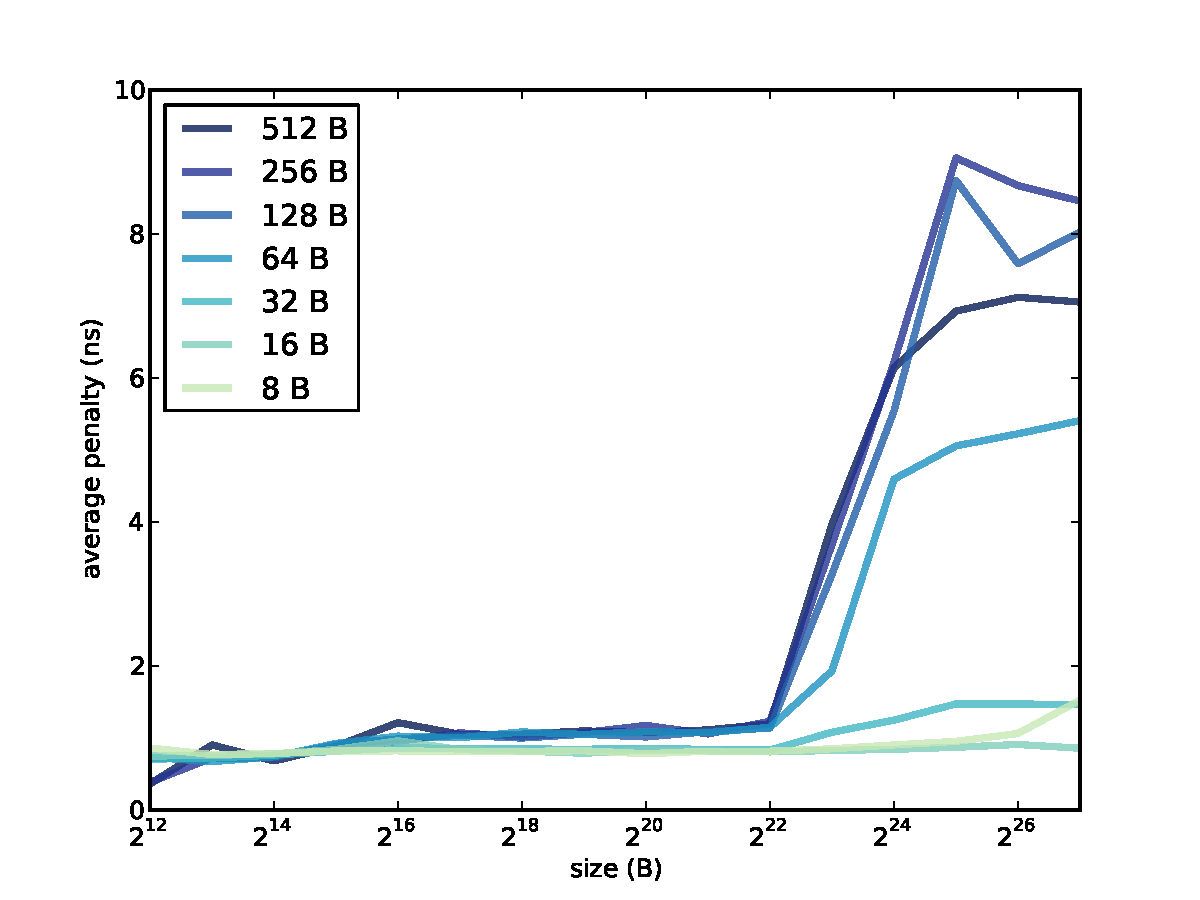
\includegraphics[width=3in]{figs/cache_data.pdf}}
\caption{Average miss penalty as a function of array size and stride.}
\label{cachedata}
\end{figure}

To isolate the time to access the elements of the array,
the program runs a second loop that is almost identical except
that the inner loop doesn't touch the array; it always increments
the same variable:

\begin{verbatim}
    iters2 = 0;
    do {
        sec0 = get_seconds();
        
        for (index = 0; index < limit; index += stride) 
            temp = temp + index;
        
        iters2 = iters2 + 1;
        sec = sec - (get_seconds() - sec0);

    } while (iters2 < iters);
\end{verbatim}

The second loop runs the same number of iterations as the first.
After each iteration, it {\em subtracts} the elapsed time from
{\tt sec}.  When the loop completes, {\tt sec} contains the total
time for all array accesses, minus the total time it took to increment
{\tt temp}.  This difference is the total miss penalty incurred by
all accesses.  Finally, we divide by the number of accesses to
get the average miss penalty per access, in ns:

\begin{verbatim}
sec * 1e9 / iters / limit * stride
\end{verbatim}

If you compile and run {\tt cache.c} you should see output like this:

\begin{verbatim}
Size:    4096 Stride:       8 read+write: 0.8633 ns
Size:    4096 Stride:      16 read+write: 0.7023 ns
Size:    4096 Stride:      32 read+write: 0.7105 ns
Size:    4096 Stride:      64 read+write: 0.7058 ns
\end{verbatim}

If you have Python and {\tt matplotlib} installed, you can use
\verb"graph_data.py" to graph the results.  Figure~\ref{cachedata}
shows the results when I ran it on a Dell Optiplex 7010.
Notice that the array size and stride are reported in
bytes, not number of array elements.

Take a minute to consider this graph, and see what you can infer
about the cache.  Here are some things to think about:

\begin{itemize}

\item The program reads through the array many times, so it has plenty
  of temporal locality.  If the entire array fits in cache, we expect
  the average miss penalty to be near 0.

\item When the stride is 4 bytes, we read every element of the array,
  so the program has plenty of spatial locality.  If the block size is
  big enough to contain 64 elements, for example, the hit rate would
  be 63/64, even if the array does not fit in cache.

\item If the stride is equal to the block size (or greater), the
  spatial locality is effectively zero, because each time we read a
  block, we only access one element.  In that case we expect to see
  the maximum miss penalty.

\end{itemize}

In summary, we expect good cache performance if the array is smaller
than the cache size {\em or} if the stride is smaller than the block
size.  Performance only degrades if the array is bigger than the
cache {\em and} the stride is large.

In Figure~\ref{cachedata}, cache performance is good, for all strides,
as long as the array is less than $2^{22}$ B.  We can infer that the
cache size is near 4 MiB; in fact, according to the specs, it is 3
MiB.

When the stride is 8, 16, or 32 B, cache performance is good.  At 64 B
it starts to degrade, and for larger strides the average miss
penalty is about 9 ns.  We can infer that the block size near 128 B.

Many processors use ``multi-level caches'' that include a small,
fast cache and a bigger, slower cache.  In this example, it looks 
like the miss penalty increases a little when the array size is bigger
than $2^{14}$ B, so it's possible that this processor also has a 16 KB
cache with an access time less than 1 ns.


\section{Programming for cache performance}

Memory caching is implemented in hardware, so most of the time
programmers don't need to know much about it.  But if you know how
caches work, you can write programs that use them more effectively.

For example, if you are working with a large array, it might be
faster to traverse the array once, performing several operations with
each element, rather than traversing the array several times.

If you are working with a 2-D array, it might be stored as an array
of rows.  If you traverse through the elements, it would be faster
to go row-wise, with stride equal to the element size, rather
than column-wise, with stride equal to the row length.

Linked data structures don't always exhibit spatial locality, because
the nodes aren't necessarily contiguous in memory.  But if you allocate
many nodes at the same time, they are usually co-located in the heap.
Or, even better, if you allocate an array of nodes all at once, you
know they will be contiguous.

Recursive strategies like mergesort often have good cache behavior
because they break big arrays into smaller pieces and then work
with the pieces.  Sometimes these algorithms can be tuned to take
advantage of cache behavior.

For applications where performance is critical, it is possible
to design algorithms tailored to the size of the cache, the block size,
and other hardware characterstics.  Algorithms like that are
called ``cache-aware''.  The obvious drawback of cache-aware
algorithms is that they are hardware-specific.


\section{The memory hierarchy}

At some point during this chapter, a question like the following
might have occurred to you: ``If caches are so much faster than
main memory, why not make a really big cache and forget about
memory?''

Without going too far into computer architecture, there are two
reasons: electronics and economics.  Caches are fast because they are
small and close to the CPU, which minimizes delays due to capacitance
and signal propagation.  If you make a cache big, it will be slower.

Also, caches take up space on the processor chip, and bigger chips are
more expensive.  Main memory is usually dynamic random-access memory
(DRAM), which uses only one transistor and one capacitor per bit, so
it is possible to pack more memory into the same amount of space.  But
this way of implementing memory is slower than the way caches are
implemented.
 
Also main memory is usually packaged in a dual in-line memory module
(DIMM) that includes 16 or more chips.  Several small chips are cheaper
than one big one.

The trade-off between speed, size, and cost is the fundamental reason
for caching.  If there were one memory technology that was fast,
big, and cheap, we wouldn't need anything else.

The same principle applies to storage as well as memory.  Solid state drives (SSD) are fast, but they are more expensive than hard drives (HDD), so they tend to be smaller.  Tape drives are even slower than hard
drives, but they can store large amounts of data relatively
cheaply.

The following table shows typical access times, sizes, and 
costs for each of these technologies.  

\vspace{0.1in}
\begin{center}
    \begin{tabular}{| l | l | l | l |}
    \hline
    Device   &   Access   &   Typical    &   Cost   \\
             &   time     &   size       &          \\ \hline
    Register &   0.5 ns   &   256 B      &   ?      \\ \hline
    Cache    &   1 ns     &   2 MiB      &   ?      \\ \hline
    DRAM     &   100 ns   &   4 GiB      &   \$10 / GiB       \\ \hline
    SSD      &   10 \mus  &   100 GiB    &   \$1 / GiB      \\ \hline
    HDD      &   5 ms     &   500 GiB    &   \$0.25 / GiB     \\ \hline
    Tape     &   minutes  &   1--2 TiB   &   \$0.02 / GiB      \\ \hline
    \end{tabular}
\end{center}
\vspace{0.1in}

The number and size of registers depends on details of the
architecture.  Current computers have about 32 general-purpose
registers, each storing one ``word''.  On a 32-bit computer, a word
is 32 bits or 4 B.  On a 64-bit computer, a word is 64 bits or 8 B.
So the total size of the register file is 100--300 B.

The cost of registers and caches is hard to quantify.  They contribute
to the cost of the chips they are on, but consumers don't see that
cost directly.

For the other numbers in the table, I looked at the specifications for
typical hardware for sale from online computer hardware stores.  By
the time you read this, these numbers will be obsolete, but they give
you an idea of what the performance and cost gaps looked like at one
point in time.

These technologies make up the ``memory hierarchy'' (note that this
use of ``memory'' also includes storage).  Each
level of the hierarchy is bigger and slower than the one above it.
And in some sense, each level acts as a cache for the one below
it.  You can think of main memory as a cache for programs and data
that are stored permanently on SSDs and HHDs.  And if you are working
with very large datasets stored on tape, you could use hard drives
to cache one subset of the data at a time.


\section{Caching policy}

The memory hierarchy suggests a framework for thinking about
caching.  At every level of the hierarchy, we have to address
four fundamental questions of caching:

\begin{itemize}

\item Who moves data up and down the hierarchy?  At the top of the
  hierarchy, register allocation is usually done by the compiler.
  Hardware on the CPU handles the memory cache.  Users implicitly move
  data from storage to memory when they execute programs and open
  files.  But the operating system also moves data back and forth
  between memory and storage.  At the bottom of the hierarchy,
  administrators move data explicitly between disk and tape.

\item What gets moved?  In general, block sizes are small at the top
  of the hierarchy and bigger at the bottom.  In a memory cache, a
  typical block size is 128 B.  Pages in memory might be 4 KiB, but
  when the operating system reads a file from disk, it might read 10s
  or 100s of blocks at a time.

\item When does data get moved?  In the most basic cache, data gets
  moved into cache when it is used for the first time.  But many
  caches use some kind of ``prefetching'', meaning that data is
  loaded before it is explicitly requested.  We have already seen
  one form of prefetching: loading an entire block when only part of
  it is requested.

\item Where in the cache does the data go?  When the cache is full, we
  can't bring anything in without kicking something out.  Ideally,
  we want to keep data that will be used again soon and replace data
  that won't.

\end{itemize}

The answers to these questions make up the ``cache policy''.
Near the top of the hierarchy, cache policies tend to be simple
because they have to be fast and they are implemented in hardware.
Near the bottom of the hierarchy, there is more time to make decisions,
and well-designed policies can make a big difference.

Most cache policies are based on the principle that history repeats
itself; if we have information about the recent past, we can use it to
predict the immediate future.  For example, if a block of data has
been used recently, we expect it to be used again soon.  This
principle suggests a replacement policy called ``least recently
used,'' or LRU, which removes from the cache a block of data that
has not been used recently.  For more on this topic, see
\url{http://en.wikipedia.org/wiki/Cache_algorithms}.


\section{Paging}
\label{paging}

In systems with virtual memory, the operating system can move
pages back and forth between memory and storage.  As I mentioned
in Section~\ref{leak}, this mechanism is called ``paging'' or
sometimes ``swapping''.

Here's how the process works:

\begin{enumerate}

\item Suppose Process A calls {\tt malloc} to allocate a chunk.  If there
is no free space in the heap with the requested size, {\tt malloc} calls
{\tt sbrk} to ask the operating system for more memory.

\item If there is a free page in physical memory, the operating system
adds it to the page table for Process A, creating a new range of valid
virtual addresses.

\item If there are no free pages, the paging system chooses a ``victim
page'' belonging to Process B.  It copies the contents of the victim
page from memory to disk, then it modifies the page table for Process
B to indicate that this page is ``swapped out''.

\item Once the data from Process B is written, the page can be reallocated
to Process A.  To prevent Process A from reading Process B's data, the
page should be cleared.

\item At this point the call to {\tt sbrk} can return, giving {\tt malloc}
additional space in the heap.  Then {\tt malloc} allocates the requested
chunk and returns.  Process A can resume.

\item When Process A completes, or is interrupted, the scheduler might
allow Process B to resume.  When Process B accesses a page that has been swapped out, the memory management unit notices that the page is ``invalid'' and causes an interrupt.

\item When the operating system handles the interrupt, it sees that
the page is swapped out, so it transfers the page back from disk to
memory.  

\item Once the page is swapped in, Process B can resume.

\end{enumerate}

When paging works well, it can greatly improve the utilization of
physical memory, allowing more processes to run in less space.
Here's why:

\begin{itemize}

\item Most processes don't use all of their allocated memory.  Many
  parts of the text segment are never executed, or execute once and
  never again.  Those pages can be swapped out without causing any
  problems.

\item If a program leaks memory, it might leave allocated space behind
  and never access it again.  By swapping those pages out, the
  operating system can effectively plug the leak.

\item On most systems, there are processes like daemons that sit idle
  most of the time and only occasionally ``wake up'' to respond to
  events.  While they are idle, these processes can be swapped out.

\item A user might have many windows open, but only a few are active
  at a time.  The inactive processes can be swapped out.

\item Also, there might be many processes running the same program.
  These processes can share the same text and static segments, avoiding the need to keep multiple copies in physical memory.

\end{itemize}

If you add up the total memory allocated to all processes, it can
greatly exceed the size of physical memory, and yet the system can
still behave well.

Up to a point.

When a process accesses a page that's swapped out, it has to get the
data back from disk, which can take several milliseconds.  The
delay is often noticeable.  If you leave a window idle for a long
time and then switch back to it, it might start slowly,
and you might hear the disk drive working while pages are
swapped in.  

Occasional delays like that might be acceptable, but if you have too
many processes using too much space, they start to interfere with each
other.  When Process A runs, it evicts the pages Process B needs.
Then when B runs, it evicts the pages A needs.  When this happens,
both processes slow to a crawl and the system can become unresponsive.
This scenario is called ``thrashing''.

In theory, operating systems could avoid thrashing by detecting an
increase in paging and blocking or killing processes until the system
is responsive again.  But as far as I can tell, most systems don't do
this, or don't do it well; it is often left to users to limit their
use of physical memory or try to recover when thrashing occurs.


\chapter{Multitasking}

In many current systems, the CPU contains multiple cores, which means
it can run several processes at the same time.  In addition, each core
is capable of ``multitasking'', which means it can switch from one
process to another quickly, creating the illusion that many processes
are running at the same time.

The part of the operating system that implements multitasking is
the ``kernel''.  In a nut or seed, the kernel is the innermost
part, surrounded by a shell.  In an operating system, the kernel
is the lowest level of software, surrounded by several other
layers, including an interface called a ``shell.''  Computer
scientists love extended metaphors.

At its most basic, the kernel's job is to
handle interrupts.  An ``interrupt'' is an event that stops the
normal instruction cycle and causes the flow of execution to jump to a
special section of code called an ``interrupt handler''.

%TODO: put new vocab in bold and add glossaries

A {\bf hardware interrupt} is caused when a device sends a signal to the
CPU.  For example, a network interface might cause an interrupt when
a packet of data arrives, or a disk drive might cause an interrupt
when a data transfer is complete.  Most systems also have timers that
cause interrupts at regular intervals, or after an elapsed time.

A {\bf software interrupt} is caused by a running program.  For example, if
an instruction cannot complete for some reason, it might trigger an
interrupt so the condition can be handled by the operating system.
Some floating-point errors, like division by zero, are handled
using interrupts.

When a program needs to access a hardware device,
it makes a {\bf system call}, which is similar to a function call,
except that instead of jumping to the beginning of the function,
it executes a special instruction that triggers an interrupt, causing
the flow of execution to jump to the kernel.  The kernel reads the
parameters of the system call, performs the requested operation,
and then resumes the interrupted process.


\section{Hardware state}

Handling interrupts requires cooperation between hardware and
software.  When an interrupt occurs, there might be several
instructions running on the CPU, data stored in registers, and
other {\bf hardware state}.

Usually the hardware is responsible for bringing the CPU
to a consistent state; for example, every instruction should either
complete or behave as if it never started.  No instruction should
be left half complete.  Also, the hardware is responsible for
saving the program counter (PC), so the kernel knows where to
resume.

Then, usually, it is the responsibility of the interrupt handler
to save the rest of the hardware state before it does anything that
might modify it, and then restore the saved state before the interrupted
process resumes.

Here is an outline of this sequence of events:

\begin{enumerate}

\item When the interrupt occurs, the hardware saves the program
counter in a special register and jumps to the appropriate interrupt
handler.

\item The interrupt handler stores the program counter and the
status register in memory, along with the contents of any data
registers it plans to use.

\item The interrupt handler runs whatever code is needed to handle
the interrupt.

\item Then it restores the contents of the saved registers.  Finally,
it restores the program counter of the interrupted process, which
has the effect of jumping back to the interrupted instruction.

\end{enumerate}

If this mechanism works correctly, there is generally no way for
the interrupted process to know there was an interrupt, unless
it detects the change in time between instructions.


\section{Context switching}

Interrupt handlers can be fast because they don't have to save the
entire hardware state; they only have to save registers they are
planning to use.

But when an interrupt occurs, the kernel does not always resume the
interrupted process.  It has the option of switching to another
process.  This mechanism is called a ``context switch''.

In general, the kernel doesn't know which registers a process will
use, so it has to save all of them.  Also, when it switches to a new
process, it might have to clear data stored in the memory management
unit (see
Section~\ref{address_translation}).  And after the context switch, it
might take some time for the new process to load data into the cache.
For these reasons, context switches are relatively slow, on the order
of thousands of cycles, or a few microseconds.

In a multi-tasking system, each process is allowed to run for a short
period of time called a ``time slice'' or ``quantum''.  During
a context switch, the kernel sets a hardware timer that causes
an interrupt at the end of the time slice.  When the interrupt
occurs, the kernel can switch to another process or allow the
interrupted process to resume.  The part of the operating system
that makes this decision is the ``scheduler''.


\section{The process life cycle}

When a process is created, the operating system allocates a
data structure that contains information about the process, called
a ``process control block'' or PCB.  Among other things, the
PCB keeps track of the process state, which is one of:

\begin{itemize}

\item Running, if the process is currently running on a core.

\item Ready, if the process could be running, but isn't, usually because
there are more runnable processes than cores.

\item Blocked, if the process cannot run because it is waiting for
a future event like network communication or a disk read.

\item Done, if the process has completed, but has exit status
information that has not been read yet.

\end{itemize}

Here are the events that cause a process to transition from one state to another:

\begin{itemize}

\item A process is created when the running program executes a system
  call like {\tt fork}.  At the end of the system call, the new
  process is usually ready.  Then the scheduler might resume the
  original process (the ``parent'') or start the new process (the
  ``child'').

\item When a process is started or resumed by the scheduler, its state
  changes from ready to running.

\item When a process is interrupted and the scheduler chooses not
  to let it resume, its state changes from running to ready.

\item If a process executes a system call that cannot complete
  immediately, like a disk request, it becomes blocked
  and the scheduler usually chooses another process.

\item When an operation like a disk request completes, it causes an
  interrupt.  The interrupt handler figures out which process was
  waiting for the request and switches its state from
  blocked to ready.  Then the scheduler may or may not choose to
  resume the unblocked process.

\item When a process calls {\tt exit}, the interrupt handler stores
  the exit code in the PCB and changes the process's state to done.

\end{itemize}


\section{Scheduling}

As we saw in Section~\ref{unixps} there might be hundreds of
processes on a computer, but usually most of them are blocked.  Most
of the time, there are only a few processes that are ready or running.
When an interrupt occurs, the scheduler decides which process to start
or resume.

On a workstation or laptop, the primary goal of the scheduler is to
minimize response time; that is, the computer should respond quickly
to user actions.  Response time is also important on a server, but in
addition the scheduler might try to maximize throughput, which is the
number of requests that complete per unit of time.

Usually the scheduler doesn't have much information about what
processes are doing, so its decisions are based on a few
heuristics:

\begin{itemize}

\item Processes might be limited by different resources.  A process
that does a lot of computation is probably CPU-bound, which means that
its run time depends on how much CPU time it gets.  A process that
reads data from a network or disk might be I/O-bound, which means that
it would run faster if data input and output went faster, but would not
run faster with more CPU time.  Finally, a process that interacts with
the user is probably blocked, most of the time, waiting for user actions.

The operating system can sometimes classify processes based on their
past behavior, and schedule them accordingly.  For example, when an
interactive process is unblocked, it should probably run immediately,
because a user is probably waiting for a reply.  On the other hand,
a CPU-bound process that has been running for a long time might be
less time-sensitive.

\item If a process is likely to run for a short time and then make
a blocking request, it should probably run immediately, for two reasons:
(1) if the request takes some time to complete, we should start it as soon
as possible, and (2) it is better for a long-running process to wait
for a short one, rather than the other way around.

As an analogy, suppose you are making an apple pie.  The crust takes
5 minutes to prepare, but then it has to chill for half an hour.  It takes
20 minutes to prepare the filling.  If you prepare the crust first,
you can prepare the filling while the crust is chilling, and you can
finish the pie in 35 minutes.  If you prepare the filling first, the
process takes 55 minutes.

\end{itemize}

Most schedulers use some form of priority-based scheduling,
where each process has a priority that can be adjusted up or down
over time.  When the scheduler runs, it chooses the runnable process
with the highest priority.

Here are some of the factors that determine a process's priority:

\begin{itemize}

\item A process usually starts with a relatively high priority so it
  starts running quickly.

\item If a process makes a request and blocks before its time slice is
  complete, it is more likely to be interactive or I/O-bound, so its
  priority should go up.

\item If a process runs for an entire time slice, it is more likely to
  be long-running and CPU-bound, so its priority should go down.

\item If a task blocks for a long time and then becomes ready, it
  should get a priority boost so it can respond to whatever it was
  waiting for.

\item If process A is blocked waiting for process B, for example if
  they are connected by a pipe, the priority of process B should go
  up.

\item The system call {\tt nice} allows a process to decrease (but not
  increase) its own priority, allowing programmers to pass explicit
  information to the scheduler.

\end{itemize}

For most systems running normal workloads, scheduling algorithms
don't have a substantial effect on performance.  Simple scheduling
policies are usually good enough.


\section{Real-time scheduling}

However, for programs that interact with the real world, scheduling
can be very important.  For example, a program that reads data from
sensors and controls motors might have to complete recurring tasks at
some minimum frequency and react to external events with some maximum
response time.  These requirements are often expressed in terms of
``tasks'' that must be completed before ``deadlines''.

Scheduling tasks to meet deadlines is called ``real-time
  scheduling''.  For some applications, a general-purpose operating
system like Linux can be modified to handle real-time scheduling.
These modifications might include:

\begin{itemize}

\item Providing richer APIs for controlling task priorities.

\item Modifying the scheduler to guarantee that the process with
highest priority runs within a fixed amount of time.

\item Reorganizing interrupt handlers to guarantee
a maximum completion time.

\item Modifying locks and other synchronization mechanisms (coming up
  in the next chapter) to allow a high-priority task to preempt a
  lower-priority task.

\item Choosing an implementation of dynamic memory allocation that
guarantees a maximum completion time.

\end{itemize}

For more demanding applications, especially in domains where real-time
response is a matter of life and death, ``real-time operating
  systems'' provide specialized capabilities, often with much simpler
designs than general purpose operating systems.

%TODO: kernel mode?  signals?  user and system time


\chapter{Threads}

When I mentioned threads in Section~\ref{unixps}, I said that a thread
is a kind of process.  Now I will provide a more careful explanation.

When you create a process, the operating system creates a new address
space, which includes the text segment, static segment, and heap; it
also creates a new ``thread of execution'', which includes the program
counter and other hardware state, and the call stack.

The processes we have seen so far are ``single-threaded'', which means
that only one thread of execution runs in each address space.  In this
chapter, you will learn about ``multi-threaded'' processes that have
multiple threads running in the same address space.

Within a single process, all threads share the same text segment, so
they run the same code.  But different threads often run different parts
of the code.

And they share the same static segment, so if one thread changes a
global variable, other threads see the change.  They also share the heap,
so threads can share dynamically-allocated chunks.

But each thread has its own stack, so threads can call functions without
interfering with each other.  Usually threads don't access each
other's local variables (and sometimes they can't).

The example code for this chapter is in the repository for this book,
in a directory named {\tt counter}.  For information on downloading
this code, see Section~\ref{code}.


\section{Creating threads}

The most popular threading standard used with C is POSIX Threads, or Pthreads for short.  The POSIX standard defines a thread model and an interface for creating and controlling threads.  Most versions of UNIX provide an implementation of Pthreads.

Using Pthreads is like using most C libraries:

\begin{itemize}

\item You include headers files at the beginning of your
program.

\item You write code that calls functions defined by Pthreads.

\item When you compile the program, you link it with the Pthread library.

\end{itemize}

For my examples, I include the following headers:

\begin{verbatim}
#include <stdio.h>
#include <stdlib.h>
#include <pthread.h>
#include <semaphore.h>
\end{verbatim}

The first two are standard; the third is for Pthreads and
the fourth is for semaphores.  To compile with the Pthread library in {\tt gcc}, you can use the {\tt -l} option on the command line:

\begin{verbatim}
gcc -g -O2 -o array array.c -lpthread
\end{verbatim}

This compiles a source file named {\tt array.c} with debugging info
and optimization, links with the Pthread library, and generates an
executable named {\tt array}.


\section{Creating threads}

The Pthread function that creates threads is called \verb"pthread_create".
The following function shows how to use it:

\begin{verbatim}
pthread_t make_thread(void *(*entry)(void *), Shared *shared)
{
    int n;
    pthread_t thread;

    n = pthread_create(&thread, NULL, entry, (void *)shared);
    if (n != 0) {
        perror("pthread_create failed");
        exit(-1);
    }
    return thread;
}
\end{verbatim}

\verb"make_thread" is a wrapper I wrote to make
\verb"pthread_create" easier to use, and to provide error-checking.

%TODO: Define a newcommand like \py to make verb easier to use, and
% get rid of the \_ hockey sticks

The return type from \verb"pthread_create" is \verb"pthread_t",
which you can think of as an id or ``handle'' for the new thread.  

If {\tt pthread\_create} succeeds, it returns 0 and \verb"make_thread"
returns the handle of the new thread.
If an error occurs, {\tt pthread\_create} 
returns an error code and \verb"make_thread" prints an error message
and exits.

The parameters of \verb"make_thread" take some
explaining.  Starting with the second, {\tt Shared}
is a structure I defined to contain values shared between threads.
The following {\tt typedef} statement creates the new type:

\begin{verbatim}
typedef struct {
    int counter;
} Shared;
\end{verbatim}

In this case, the only shared variable is {\tt counter}.
{\tt make\_shared} allocates
space for a {\tt Shared} structure and initializes the contents:

\begin{verbatim}
Shared *make_shared()
{
    Shared *shared = check_malloc(sizeof (Shared));
    shared->counter = 0;
    return shared;
}
\end{verbatim}

Now that we have a shared data structure, let's get back to
\verb"make_thread".
The first parameter is a pointer to a function that takes
a {\tt void} pointer and returns a {\tt void} pointer.  If the syntax
for declaring this type makes your eyes bleed, you are not alone.
Anyway, the purpose of this parameter is to specify the function where
the execution of the new thread will begin.  By convention, this
function is named {\tt entry}:

\begin{verbatim}
void *entry(void *arg)
{
    Shared *shared = (Shared *) arg;
    child_code(shared);
    pthread_exit(NULL);
}
\end{verbatim}

The parameter of {\tt entry} has to be declared as a {\tt void}
pointer, but in this program we know that it is really a pointer to a
{\tt Shared} structure, so we can typecast it accordingly and then
pass it along to {\tt child\_code}, which does the real work.

As a simple example, \verb"child_code" prints the value of
the shared counter and increments it.

\begin{verbatim}
void child_code(Shared *shared)
{  
    printf("counter = %d\n", shared->counter);
    shared->counter++;
}
\end{verbatim}

When {\tt child\_code} returns, {\tt entry} invokes
\verb"pthread_exit" which can be used to pass a value to the thread
that joins with this thread.  In this case, the child has nothing to
say, so we pass {\tt NULL}.

Finally, here is the code that creates the child threads:

\begin{verbatim}
    int i;
    pthread_t child[NUM_CHILDREN];

    Shared *shared = make_shared(1000000);

    for (i=0; i<NUM_CHILDREN; i++) {
        child[i] = make_thread(entry, shared);
    }
\end{verbatim}

\verb"NUM_CHILDREN" is a compile-time constant that determines
the number of child threads.  {\tt child} is an array of
thread handles.


\section{Joining threads}

When one thread wants to wait for another thread to complete,
it invokes {\tt pthread\_join}.
Here is my wrapper for {\tt pthread\_join}:

\begin{verbatim}
void join_thread(pthread_t thread)
{
    int ret = pthread_join(thread, NULL);
    if (ret == -1) {
      perror("pthread_join failed");
      exit(-1);
    }
}
\end{verbatim}

The parameter is the handle of the thread you want to wait for.
All the wrapper does is call {\tt pthread\_join} and check the
result.

Any thread can join any other thread, but in the most common pattern
the parent thread creates and joins all child threads.
Continuing the example from the previous section, here's the
code that waits on the children:

\begin{verbatim}
    for (i=0; i<NUM_CHILDREN; i++) {
        join_thread(child[i]);
    }
\end{verbatim}

This loops waits for the children one at a time in the order they
were created.  There is no guarantee that the child threads complete 
in that order, but this loop works correctly even if they don't.  If one
of the children is late, the loop might have to wait, and other children
might complete in the meantime.  But regardless, the loop exits
only when all children are done.

If you have downloaded the repository for this book (see
Section~\ref{code}), you'll find this example in {\tt
  counter/counter.c}.  You can compile and run it like this:

\begin{verbatim}
$ make counter
gcc -Wall counter.c -o counter -lpthread
$ ./counter
\end{verbatim}

When I ran it with 5 children, I got the following output:

\begin{verbatim}
counter = 0
counter = 0
counter = 1
counter = 0
counter = 3
\end{verbatim}

When you run it, you will probably get different results.  And if
you run it again, you might get different results each time.  What's
going on?


\section{Synchronization errors}

The problem with the previous program is that the children
access the shared variable, {\tt counter}, without synchronization,
so several threads can read the same value of {\tt counter} before
any threads increment it.

Here is a sequence of events that could explain the output in the
previous section:

\begin{verbatim}
Child A reads 0
Child B reads 0
Child C reads 0
Child A prints   0
Child B prints   0
Child A sets counter=1
Child D reads 1
Child D prints   1
Child C prints   0
Child A sets counter=1
Child B sets counter=2
Child C sets counter=3
Child E reads 3
Child E prints   3
Child D sets counter=4
Child E sets counter=5
\end{verbatim}

Each time you run the program, threads might be interrupted at different
points, or the scheduler might choose different threads to run, so
the sequence of events, and the results, will be different.

Suppose we want to impose some order.  For example, we might want
each thread to read a different value of {\tt counter} and increment
it, so that the value of {\tt counter} reflects the number of
threads that have executed \verb"child_code".

To enforce that requirement, we can use a ``mutex'', which is
an object that guarantees ``mutual exclusion'' for a block of code;
that is, only one thread can execute the block at a time.

I have written a small module called {\tt mutex.c} that provides
mutex objects.  I'll show you how to use it first; then I'll explain
how it works.

Here's a version of \verb"child_code" that uses a mutex to synchronize
threads:

\begin{verbatim}
void child_code(Shared *shared)
{
    mutex_lock(shared->mutex);
    printf("counter = %d\n", shared->counter);
    shared->counter++;
    mutex_unlock(shared->mutex);
}
\end{verbatim}

Before any thread can access {\tt counter}, it has to ``lock''
the mutex, which has the effect of barring all other threads.
Suppose Thread A has locked the mutex and is in the
middle of \verb"child_code".  If Thread B arrives and
executes \verb"mutex_lock", it blocks.

When Thread A is done, it executes \verb"mutex_unlock",
which allows Thread B to proceed.  In effect, the threads
line up to execute \verb"child_code" one at a time, so they
can't interfere with each other.  When I run this code with
5 children, I get:

\begin{verbatim}
counter = 0
counter = 1
counter = 2
counter = 3
counter = 4
\end{verbatim}

And that satisfies the requirements.  In order for this solution to
work, I have to add the Mutex to the Shared struct:

\begin{verbatim}
typedef struct {
    int counter;
    Mutex *mutex;
} Shared;
\end{verbatim}

And initialize it in \verb"make_shared"

\begin{verbatim}
Shared *make_shared(int end)
{
    Shared *shared = check_malloc(sizeof(Shared));
    shared->counter = 0;
    shared->mutex = make_mutex();   //-- this line is new
    return shared;
}
\end{verbatim}

The code in this section is in \verb"counter_mutex.c".
The definition of {\tt Mutex} is in {\tt mutex.c}, which I
explain in the next section.



\section{Mutex}

My definition of {\tt Mutex} is a wrapper for a type called
\verb"pthread_mutex_t", which is defined in the POSIX threads API.

To create a POSIX mutex, you have to allocate space for a
\verb"pthread_mutex_t" type and then call \verb"pthread_mutex_init".

One of the problems with this API is that \verb"pthread_mutex_t"
behaves like a structure, so if you pass it as an argument, it makes a
copy, which makes the mutex behave incorrectly.  To avoid that, you have to
pass \verb"pthread_mutex_t" by address.

My code makes it easier to get that right.  It defines a
type, {\tt Mutex}, which is just a more readable name for
\verb"pthread_mutex_t":

\begin{verbatim}
#include <pthread.h>

typedef pthread_mutex_t Mutex;
\end{verbatim}

Then it defines \verb"make_mutex", which allocates space and
initializes the mutex:

\begin{verbatim}
Mutex *make_mutex()
{
    Mutex *mutex = check_malloc(sizeof(Mutex));
    int n = pthread_mutex_init(mutex, NULL);
    if (n != 0) perror_exit("make_lock failed"); 
    return mutex;
}
\end{verbatim}

The return value is a pointer, which you can pass around as an
argument without causing unwanted copying.

The functions to lock and unlock the mutex are simple wrappers
for POSIX functions:

\begin{verbatim}
void mutex_lock(Mutex *mutex)
{
    int n = pthread_mutex_lock(mutex);
    if (n != 0) perror_exit("lock failed");
}

void mutex_unlock(Mutex *mutex)
{
    int n = pthread_mutex_unlock(mutex);
    if (n != 0) perror_exit("unlock failed");
}
\end{verbatim}

This code is in {\tt mutex.c} and the header file {\tt mutex.h}.


\chapter{Condition variables}
\label{csem}

Many simple synchronization problems can be solved using mutexes
as shown in the previous chapter.  In this chapter I introduce a
bigger challenge, the well-known ``Producer-Consumer problem'', and
a new tool to solve it, the condition variable.

\section{The work queue}
\label{queue}

In some multi-threaded programs, threads are organized to perform
different tasks.  Often they communicate with each other using a queue,
where some threads, called ``producers'', put data into the queue
and other threads, called ``consumers'', take data out.

For example, in applications with a graphical user interface, there
might be one thread that runs the GUI, responding to user events,
and another thread that processes user requests.  In that case,
the GUI thread might put requests into a queue and the ``back end''
thread might take requests out and process them.

To support this organization, we need a queue implementation that is
``thread safe'', which means that both threads (or more than two) can
access the queue at the same time.  And we need to handle the special
cases when the queue is empty and, if the size of the queue is
bounded, when the queue is full.

I'll start with a simple queue that is not thread safe, then we'll see
what goes wrong and fix it.  The code for this example is in the
repository for this book, in a folder called {\tt queue}.  The file
{\tt queue.c} contains a basic implementation of a circular buffer,
which you can read about at
\url{https://en.wikipedia.org/wiki/Circular_buffer}.

Here's the structure definition:

\begin{verbatim}
typedef struct {
    int *array;
    int length;
    int next_in;
    int next_out;
} Queue;
\end{verbatim}

{\tt array} is the array that contains the elements of the queue.
For this example the elements are ints, but more generally
they would be structures that contain user events, items of work, etc.

{\tt length} is the length of the array.  \verb"next_in" is an
index into the array that indices where the next element should be
added; similarly, \verb"next_out" is the index of the next element
that should be removed.

\verb"make_queue" allocates space for this structure and initializes
the fields:

\begin{verbatim}
Queue *make_queue(int length)
{
    Queue *queue = (Queue *) malloc(sizeof(Queue));
    queue->length = length + 1;
    queue->array = (int *) malloc(length * sizeof(int));
    queue->next_in = 0;
    queue->next_out = 0;
    return queue;
}
\end{verbatim}

The initial value for \verb"next_out" needs some explaining.
Since the queue is initially empty, there is no next element to
remove, so \verb"next_out" is invalid.  Setting
\verb"next_out == next_in" is a special case that indicates
that the queue is empty, so we can write:

\begin{verbatim}
int queue_empty(Queue *queue)
{
    return (queue->next_in == queue->next_out);
}
\end{verbatim}

Now we can add elements to the queue using \verb"queue_push":

\begin{verbatim}
void queue_push(Queue *queue, int item) {
    if (queue_full(queue)) {
        perror_exit("queue is full");
    }
  
    queue->array[queue->next_in] = item;
    queue->next_in = queue_incr(queue, queue->next_in);
}
\end{verbatim}

If the queue is full, \verb"queue_push" prints an error message
and exits.  I will explain \verb"queue_full" soon.

If the queue is not full, \verb"queue_push" inserts the new
element and then increments \verb"next_in" using \verb"queue_incr":

\begin{verbatim}
int queue_incr(Queue *queue, int i)
{
    return (i+1) % queue->length;
}
\end{verbatim}

When the index, {\tt i}, gets to the end of the array, it wraps around
to 0.  And that's where we run into a tricky part.  If we keep adding
elements to the queue, eventually \verb"next_in" wraps around and catches
up with \verb"next_out".  But if \verb"next_in == next_out", we would
incorrectly conclude that the queue was empty.

To avoid that, we define another special case to indicate that the
queue is full:

\begin{verbatim}
int queue_full(Queue *queue)
{
    return (queue_incr(queue, queue->next_in) == queue->next_out);
}
\end{verbatim}

If incrementing \verb"next_in" lands on \verb"next_out", that means
we can't add another element without making the queue seem empty.  So
we stop one element before the ``end'' (keeping in mind that the end of
the queue can be anywhere, not necessarily the end of the array).

Now we can write \verb"queue_pop", which removes and returns the next
element from the queue:

\begin{verbatim}
int queue_pop(Queue *queue) {
    if (queue_empty(queue)) {
        perror_exit("queue is empty");
    }
  
    int item = queue->array[queue->next_out];
    queue->next_out = queue_incr(queue, queue->next_out);
    return item;
}
\end{verbatim}

If you try to pop from an empty queue, \verb"queue_pop" prints
an error message and exits.


\section{Producers and consumers}
\label{prodcon}

Now let's make some threads to access this queue.  Here's the
producer code:

\begin{verbatim}
void *producer_entry(void *arg) {
    Shared *shared = (Shared *) arg;

    for (int i=0; i<QUEUE_LENGTH-1; i++) {
        printf("adding item %d\n", i);
        queue_push(shared->queue, i);
    }
    pthread_exit(NULL);
}
\end{verbatim}

Here's the consumer code:

\begin{verbatim}
void *consumer_entry(void *arg) {
    int item;
    Shared *shared = (Shared *) arg;

    for (int i=0; i<QUEUE_LENGTH-1; i++) {
        item = queue_pop(shared->queue);
        printf("consuming item %d\n", item);
    }
    pthread_exit(NULL);
}
\end{verbatim}

Here's the parent code that starts the threads and waits for them

\begin{verbatim}
    pthread_t child[NUM_CHILDREN];

    Shared *shared = make_shared();

    child[0] = make_thread(producer_entry, shared);
    child[1] = make_thread(consumer_entry, shared);

    for (int i=0; i<NUM_CHILDREN; i++) {
        join_thread(child[i]);
    }
\end{verbatim}

And finally here's the shared structure that contains the queue:

\begin{verbatim}
typedef struct {
    Queue *queue;
} Shared;

Shared *make_shared()
{
    Shared *shared = check_malloc(sizeof(Shared));
    shared->queue = make_queue(QUEUE_LENGTH);
    return shared;
}
\end{verbatim}

The code we have so far is a good starting place, but it has
several problems:

\begin{itemize}

\item Access to the queue is not thread safe.  Different threads
could access {\tt array}, \verb"next_in", and \verb"next_out"
at the same time and leave the queue in a broken, ``inconsistent''
state.

\item If the consumer is scheduled first, it finds the queue empty,
print an error message, and exits.  We would rather have the consumer
block until the queue is not empty.  Similarly, we would like the
producer to block if the queue is full.

\end{itemize}

In the next section, we solve the first problem with a {\tt Mutex}.
In the following section, we solve the second problem with condition
variables.


\section{Mutual exclusion}

We can make the queue thread safe with a mutex.  This version
of the code is in \verb"queue_mutex.c".

First we add a {\tt Mutex} pointer to the queue structure:

\begin{verbatim}
typedef struct {
    int *array;
    int length;
    int next_in;
    int next_out;
    Mutex *mutex;          //-- this line is new
} Queue;
\end{verbatim}

And initialize the {\tt Mutex} in \verb"make_queue":

\begin{verbatim}
Queue *make_queue(int length) {
    Queue *queue = (Queue *) malloc(sizeof(Queue));
    queue->length = length;
    queue->array = (int *) malloc(length * sizeof(int));
    queue->next_in = 0;
    queue->next_out = 0;
    queue->mutex = make_mutex();   //-- new
    return queue;
}
\end{verbatim}

Next we add synchronization code to \verb"queue_push":

\begin{verbatim}
void queue_push(Queue *queue, int item) {
    mutex_lock(queue->mutex);   //-- new
    if (queue_full(queue)) {
      mutex_unlock(queue->mutex);   //-- new
      perror_exit("queue is full");
    }
  
    queue->array[queue->next_in] = item;
    queue->next_in = queue_incr(queue, queue->next_in);
    mutex_unlock(queue->mutex);   //-- new
}
\end{verbatim}

Before checking whether the queue is full, we have to lock
the {\tt Mutex}.  If the queue is full, we have to unlock
the {\tt Mutex} before exiting; otherwise the thread would leave
it locked and no other threads could proceed.

The synchronization code for \verb"queue_pop" is similar:

\begin{verbatim}
int queue_pop(Queue *queue) {
    mutex_lock(queue->mutex);
    if (queue_empty(queue)) {
      mutex_unlock(queue->mutex);
      perror_exit("queue is empty");
    }
  
    int item = queue->array[queue->next_out];
    queue->next_out = queue_incr(queue, queue->next_out);
    mutex_unlock(queue->mutex);
    return item;
}
\end{verbatim}

Note that the other {\tt Queue} functions, \verb"queue_full",
\verb"queue_empty", and \verb"queue_incr" do not try to lock
the mutex.  Any thread that calls these functions is required to
lock the mutex first; this requirement is part of the documented
interface for these functions.

With this additional code, the queue is thread safe; if you run it, you
should not see any synchronization errors.  But it is likely
that the consumer will exit at some point because the queue is
empty, or the producer will exit because the queue is full,
or both.

The next step is to add condition variables.


\section{Condition variables}

A condition variable is a data structure associated with a condition;
it allows threads to block until the condition becomes true.  For
example, \verb"thread_pop" might want check whether the queue is
empty and, if so, wait for a condition like ``queue not empty''.

Similarly, \verb"thread_push" might want to check whether the queue is
full and, if so, block until it is not full.

I'll handle the first condition here, and you will have a chance to
handle the second condition as an exercise.

First we add a condition variable to the {\tt Queue} structure:

\begin{verbatim}
typedef struct {
    int *array;
    int length;
    int next_in;
    int next_out;
    Mutex *mutex;
    Cond *nonempty;   //-- new
} Queue;
\end{verbatim}

And initialize it in \verb"make_queue":

\begin{verbatim}
Queue *make_queue(int length)
{
    Queue *queue = (Queue *) malloc(sizeof(Queue));
    queue->length = length;
    queue->array = (int *) malloc(length * sizeof(int));
    queue->next_in = 0;
    queue->next_out = 0;
    queue->mutex = make_mutex();
    queue->nonempty = make_cond();   //-- new
    return queue;
}
\end{verbatim}

Now in \verb"queue_pop", if we find the queue empty, we don't
exit; instead we use the condition variable to block:

\begin{verbatim}
int queue_pop(Queue *queue) {
  mutex_lock(queue->mutex);
  while (queue_empty(queue)) {
    cond_wait(queue->nonempty, queue->mutex);  //-- new
  }
  
  int item = queue->array[queue->next_out];
  queue->next_out = queue_incr(queue, queue->next_out);
  mutex_unlock(queue->mutex);
  cond_signal(queue->nonfull);   //-- new
  return item;
}
\end{verbatim}

\verb"cond_wait" is complicated, so let's take it slow.  
The first argument is the condition variable; in this case,
the condition we are waiting for is ``queue not empty''.  The second
argument is the mutex that protects the queue.

When the thread that locked the mutex calls \verb"cond_wait", it
unlocks the mutex and then blocks.  This is important.  If
\verb"cond_wait" did not unlock the mutex before blocking, no
other thread would be able to access the queue, no more items
could be added, and the queue would always be empty.

So while the consumer is blocked on {\tt nonempty}, the producer can
run.  Let's see what happens when the producer runs \verb"queue_push":

\begin{verbatim}
void queue_push(Queue *queue, int item) {
    mutex_lock(queue->mutex);
    if (queue_full(queue)) {
        mutex_unlock(queue->mutex);
        perror_exit("queue is full");
    }
    queue->array[queue->next_in] = item;
    queue->next_in = queue_incr(queue, queue->next_in);
    mutex_unlock(queue->mutex);
    cond_signal(queue->nonempty);    //-- new
}
\end{verbatim}

Just as before, \verb"queue_push" locks the {\tt Mutex} and checks
whether the queue is full.  Assuming it is not, \verb"queue_push" adds
a new element to the queue and then unlocks the {\tt Mutex}.

But before returning, it does one more thing: it ``signals'' the
condition variable {\tt nonempty}.

Signalling a condition variable usually indicates that the condition is
true.  If there are no threads waiting
on the condition variable, the signal has no effect.

If there are threads waiting on the condition variable, one of them
gets unblocked and resumes execution of \verb"cond_wait".  But before
the awakened thread can return from \verb"cond_wait", it has
to wait for and lock the {\tt Mutex}, again.

Now go back to \verb"queue_pop" and see what happens when the thread
returns from \verb"cond_wait".  It loops back to the top of the while
loop and checks the condition again.  I'll explain why in just a
second, but for now let's assume that the condition is true; that is,
the queue is not empty.

When the consumer thread exits the while loop, we know two things: (1)
the condition is true, so there is at least one item in the queue, and
(2) the {\tt Mutex} is locked, so it is safe to access the queue.

After removing an item, \verb"queue_pop" unlocks the mutex
and returns.

In the next section I'll show you how my {\tt Cond} code works, but first I
want to answer two frequently-asked questions:

\begin{itemize}

\item Why is \verb"cond_wait" inside a while loop rather than an if
statement; that is, why do we have to check the condition again after
returning from \verb"cond_wait"?

The primary reason you have to re-check the condition is the possibility
of an intercepted signal.  Suppose Thread A is waiting on {\tt nonempty}.
Thread B adds an item to the queue and signals {\tt nonempty}.  Thread
A wakes up an tries to lock the mutex, but before it gets the chance,
Evil Thread C swoops in, locks the mutex, pops the item from the
queue, and unlocks the mutex.  Now the queue is empty again, but
Thread A is not blocked any more.  Thread A could lock the mutex and
returns from \verb"cond_wait".  If Thread A does not check the condition
again, it would try to pop an element from an empty queue, and probably
cause an error.

\item The other question that comes up when people learn about condition
variables is ``How does the condition variable know what condition it
is associated with?''

This question is understandable because there is no explicit connection
between a {\tt Cond} structure and the condition it relates to.  The
connection is implicit in the way it is used.

Here's one way to think of it: the condition associated with a Cond
is the thing that is false when you call \verb"cond_wait" and true
when you call \verb"cond_signal".

\end{itemize}

Because threads have to check the condition when they return from
\verb"cond_wait", it is not strictly necessary to call \verb"cond_signal"
only when the condition is true.  If you have reason to think the
condition {\em might} be true, you could call \verb"cond_signal" as
a suggestion that now is a good time to check.


\section{Condition variable implementation}

The Cond structure I used in the previous section is a wrapper
for a type called \verb"pthread_cond_t", which is defined in the POSIX
threads API.  It is very similar to Mutex, which is a wrapper for
\verb"pthread_mutex_t".  Both wrappers are defined in {\tt utils.c} and
{\tt utils.h}.

Here's the typedef:

\begin{verbatim}
typedef pthread_cond_t Cond;
\end{verbatim}

\verb"make_cond" allocates space, initializes the condition variable,
and returns a pointer:

\begin{verbatim}
Cond *make_cond() {
    Cond *cond = check_malloc(sizeof(Cond)); 
    int n = pthread_cond_init(cond, NULL);
    if (n != 0) perror_exit("make_cond failed");
 
    return cond;
}
\end{verbatim}

And here are the wrappers for \verb"cond_wait" and \verb"cond_signal".

\begin{verbatim}
void cond_wait(Cond *cond, Mutex *mutex) {
    int n = pthread_cond_wait(cond, mutex);
    if (n != 0) perror_exit("cond_wait failed");
}

void cond_signal(Cond *cond) {
    int n = pthread_cond_signal(cond);
    if (n != 0) perror_exit("cond_signal failed");
}
\end{verbatim}

At this point there should be nothing too surprising there.



\chapter{Semaphores in C}

Semaphores are a good way to learn about synchronization, but
they are not as widely used, in practice, as mutexes and
condition variables.

Nevertheless, there are some synchronization problems that can be
solved simply with semaphores, yielding solutions that are more
demonstrably correct.

This chapter presents a C API for working with semaphores and
my code for making it easier to work with.  And it presents
a final challenge: can you write an implementation of a semaphore
using mutexes and condition variables?

The code for this chapter is in directory {\tt semaphore} in the
repository for this book (see Section~\ref{code}).


\section{POSIX Semaphores}

A semaphore is a data structure used to help threads work together
without interfering with each other.

The POSIX standard specifies an interface for semaphores;
it is not part of Pthreads, but most UNIXes
that implement Pthreads also provide semaphores.

POSIX semaphores have type {\tt sem\_t}.
As usual, I put a wrapper around {\tt sem\_t}
to make it easier to use.  The interface is defined in {\tt sem.h}:

\begin{verbatim}
typedef sem_t Semaphore;

Semaphore *make_semaphore(int value);
void semaphore_wait(Semaphore *sem);
void semaphore_signal(Semaphore *sem);
\end{verbatim}

{\tt Semaphore} is a synonym for \verb"sem_t", but I find it more
readable, and the capital letter reminds me to treat it like an
object and pass it by pointer.

The implementation of these functions is in {\tt sem.c}:

\begin{verbatim}
Semaphore *make_semaphore(int value)
{
    Semaphore *sem = check_malloc(sizeof(Semaphore));
    int n = sem_init(sem, 0, value);
    if (n != 0) perror_exit("sem_init failed");
    return sem;
}
\end{verbatim}

{\tt make\_semaphore} takes the initial value of the semaphore
as a parameter.  It allocates space for a Semaphore, initializes
it, and returns a pointer to {\tt Semaphore}.

{\tt sem\_init} returns 0 if it succeeds and -1 if anything goes
wrong.  One nice thing about using wrapper functions is that you can
encapsulate the error-checking code, which makes the code that uses
these functions more readable.

Here is the implementation of \verb"semaphore_wait":

\begin{verbatim}
void semaphore_wait(Semaphore *sem)
{
    int n = sem_wait(sem);
    if (n != 0) perror_exit("sem_wait failed");
}
\end{verbatim}

And here is \verb"semaphore_signal":

\begin{verbatim}
void semaphore_signal(Semaphore *sem)
{
    int n = sem_post(sem);
    if (n != 0) perror_exit("sem_post failed");
}
\end{verbatim}

I prefer to call this operation ``signal'' rather than ``post'',
although both terms are common.

Here's an example that shows how to use a semaphore as a mutex:

\begin{verbatim}
Semaphore *mutex = make_semaphore(1);

semaphore_wait(mutex);
  // protected code goes here
semaphore_signal(mutex);
\end{verbatim}

When you use a semaphore as a mutex, you usually
initialize it to 1 to indicate
that the mutex is unlocked; that is, one thread can
pass the semaphore without blocking.

Here I am using the variable name {\tt mutex} to indicate that
the semaphore is being used as a mutex.  But remember that the behavior
of a semaphore is not the same as a Pthread mutex.


\section{Producers and consumers with semaphores}

Using these semaphore wrapper functions, we can
write a solution to the Producer-Consumer problem from
Section~\ref{prodcon}.
The code in this section is in \verb"queue_sem.c".

Here's the new definition of {\tt Queue}, replacing the mutex
and condition variables with semaphores:

\begin{verbatim}
typedef struct {
    int *array;
    int length;
    int next_in;
    int next_out;
    Semaphore *mutex;       //-- new
    Semaphore *items;       //-- new
    Semaphore *spaces;      //-- new
} Queue;
\end{verbatim}

And here's the new version of \verb"make_queue":

\begin{verbatim}
Queue *make_queue(int length)
{
    Queue *queue = (Queue *) malloc(sizeof(Queue));
    queue->length = length;
    queue->array = (int *) malloc(length * sizeof(int));
    queue->next_in = 0;
    queue->next_out = 0;
    queue->mutex = make_semaphore(1);
    queue->items = make_semaphore(0);
    queue->spaces = make_semaphore(length-1);
    return queue;
}
\end{verbatim}

{\tt mutex} is used to guarantee exclusive access to the queue;
the initial value is 1, so the mutex is
initially unlocked.

{\tt items} is the number of items in the queue, which is also the number
of consumer threads that can execute \verb"queue_pop" without blocking.
Initially there are no items in the queue.

{\tt spaces} is the number of empty spaces in the queue, which is the
number of producer threads that can execute \verb"queue_push" without
blocking.  Initially the number of spaces is the capacity of the queue,
which is {\tt length-1}, as explained in Section~\ref{queue}.

Here is the new version of \verb"queue_push", which is run by
producer threads:

\begin{verbatim}
void queue_push(Queue *queue, int item) {
  semaphore_wait(queue->spaces);
  semaphore_wait(queue->mutex);

  queue->array[queue->next_in] = item;
  queue->next_in = queue_incr(queue, queue->next_in);

  semaphore_signal(queue->mutex);
  semaphore_signal(queue->items);
}
\end{verbatim}

Notice that \verb"queue_push" doesn't have to call
\verb"queue_full" any more; instead, the semaphore keeps track of
how many spaces are available and blocks producers if the queue
is full.

Here is the new version of \verb"queue_pop":

\begin{verbatim}
int queue_pop(Queue *queue) {
  semaphore_wait(queue->items);
  semaphore_wait(queue->mutex);
  
  int item = queue->array[queue->next_out];
  queue->next_out = queue_incr(queue, queue->next_out);

  semaphore_signal(queue->mutex);
  semaphore_signal(queue->spaces);

  return item;
}
\end{verbatim}

This solution is explained, using pseudo-code, in Chapter 4 of
{\it The Little Book of Semaphores}.

Using the code in the repository for this book, you should be able to compile and run this solution like this:

\begin{verbatim}
$ make queue_sem
$ ./queue_sem
\end{verbatim}



\section{Make your own semaphores}
\label{makeyourown}

Any problem that can be solved with semaphores can also be solved
with condition variables and mutexes.  We can prove that's true
by using condition variables and mutexes to implement a semaphore.

Before you go on, you might want to try this as an exercise: write
functions that implement the semaphore API in {\tt sem.h}
using using condition variables and mutexes.  In the repository for this book, you'll find my solution in \verb"mysem_soln.c" and
\verb"mysem_soln.h".

If you have trouble getting started, you can use the following
structure definition, from my solution, as a hint:

\begin{verbatim}
typedef struct {
  int value, wakeups;
  Mutex *mutex;
  Cond *cond;
} Semaphore;
\end{verbatim}

% TODO: Include Property 3 (it's in LBoS).

{\tt value} is the value of the semaphore.  {\tt wakeups} counts
the number of pending signals; that is, the number of threads
that have been woken but have not yet resumed execution.  The reason
for wakeups is to make sure that our semaphores have
Property 3, described in {\tt The Little Book of Semaphores}.

{\tt mutex} provides exclusive access to {\tt value} and
{\tt wakeups}; {\tt cond} is the condition variable threads
wait on if they wait on the semaphore.

Here is the initialization code for this structure:

\begin{verbatim}
Semaphore *make_semaphore(int value)
{
  Semaphore *semaphore = check_malloc(sizeof(Semaphore));
  semaphore->value = value;
  semaphore->wakeups = 0;
  semaphore->mutex = make_mutex();
  semaphore->cond = make_cond();
  return semaphore;
}
\end{verbatim}


\subsection{Semaphore implementation}

Here is my implementation of semaphores using POSIX mutexes
and condition variables:

\begin{verbatim}
void semaphore_wait(Semaphore *semaphore)
{
  mutex_lock(semaphore->mutex);
  semaphore->value--;

  if (semaphore->value < 0) {
    do {
      cond_wait(semaphore->cond, semaphore->mutex);
    } while (semaphore->wakeups < 1);
    semaphore->wakeups--;
  }
  mutex_unlock(semaphore->mutex);
}
\end{verbatim}

When a thread waits on the semaphore, it has to lock the mutex
before it decrements {\tt value}.  If the value of the semaphore
becomes negative, the thread blocks until a ``wakeup'' is
available.  While it is blocked, the mutex is unlocked, so another
thread can signal.

Here is the code for \verb"semaphore_signal":

\begin{verbatim}
void semaphore_signal(Semaphore *semaphore)
{
  mutex_lock(semaphore->mutex);
  semaphore->value++;

  if (semaphore->value <= 0) {
    semaphore->wakeups++;
    cond_signal(semaphore->cond);
  }
  mutex_unlock(semaphore->mutex);
}
\end{verbatim}

Again, a thread has to lock the mutex before it increments
{\tt value}.  If the semaphore was negative, that means threads
are waiting, so the signalling thread increments {\tt wakeups} and
signals the condition variable.

At this point one of the waiting threads might wake up, but the
mutex is still locked until the signalling thread unlocks it.

At that point, one of the waiting threads returns from \verb"cond_wait"
and checks whether a wakeup is still available.  If not, it
loops and waits on the condition variable again.  If so, it
decrements {\tt wakeups}, unlocks the mutex, and exits.

One thing about this solution that might not be obvious is the use of
a {\tt do...while} loop.  Can you figure out why it is not a
more conventional {\tt while} loop?  What would go wrong?

The problem is that with a {\tt while} loop this implementation would
not have Property 3.  It would be possible for a thread to signal and
then run around and catch its own signal.

With the {\tt do...while} loop, it is guaranteed\footnote{Well,
  almost.  It turns out that a well-timed spurious wakeup (see
  \url{http://en.wikipedia.org/wiki/Spurious_wakeup}) can violate this
  guarantee.} that when a thread signals, one of the waiting threads
will get the signal, even if the signalling thread runs around and
gets the mutex before one of the waiting threads resumes.

\end{document}


